%! TEX TS-program = xelatex

\documentclass[a4paper,10pt]{article}

% Подключение библиотек
\usepackage{geometry}
\usepackage{lipsum}
\usepackage{fancyhdr}
\usepackage{fontspec}
\usepackage{setspace}
\usepackage{ulem}
\usepackage{indentfirst}
\usepackage[english, russian]{babel}
\usepackage[hidelinks]{hyperref}
\usepackage{graphicx}
\usepackage{amsmath}
\usepackage{totcount}
\usepackage{calc}
\usepackage{tabularx}
\usepackage{ifthen}
\usepackage{threeparttable}
\usepackage{float}

% Установка пути картинок
\graphicspath{ {./images/} {./images.example/} }

% Установка базового шрифта (Требуется XeLatex)
\setmainfont{Times New Roman}

% Подключение файлов. В них возможны подключения библиотек. Поэтому выше список используемых  библиотек не полон.
% Файл с константами документа
\IfFileExists{./constants.tex}{
    % Константы

% Тема
\newcommand{\topic}{Разработка конструктора Telegram-ботов. Часть 1}

% ТПЖА
\newcommand{\tpga}{TПЖА 09.03.01.514}

% Тип документа
\newcommand{\doctype}{ДДП}

% Кафедра и группа
\newcommand{\departmentandgroupinframe}{Кафедра ЭВМ Группа ИВТ-41}

% Разработал
\newcommand{\authorinframe}{Бушков}

% Проверяющий
\newcommand{\inspectorinframe}{Долженкова}

% Нормоконтролер
\newcommand{\norminspectorinframe}{Скворцов}

% Утверждающий
\newcommand{\approverinframe}{Долженкова}

}{
    % Константы

% Тема
\newcommand{\topic}{Разработка машины времени}
% Фамилия автора документа
\newcommand{\authorsecondname}{Волков}
% Фамилия с инициалами
\newcommand{\authorwithinitials}{
	\authorsecondname~М.~В.}


% ТПЖА
\newcommand{\tpga}{TПЖА 09.03.01.514~ПЗ}
% Направление
\newcommand{\specialization}{09.03.01 - Информатика и вычислительная техника}
% Профиль
\newcommand{\profile}{Программное и аппаратное обеспечение вычислительной техники}

% Студент. Группа
\newcommand{\studentgroup}{студент гр.ИВТб-4301-04-00}

% Заведующая кафедрой
\newcommand{\headofdepartment}{Долженкова М. Л.}

% Руководитель
\newcommand{\supervisor}{Долженкова М. Л.}

% Звание руководителя
\newcommand{\supervisorrank}{\\ к.т.н., доцент, зав. кафедрой ЭВМ}

% Указание консультанта
\newboolean{consultantexists}
\setboolean{consultantexists}{True}

% Консультант
\newcommand{\consultant}{Кошкин О. В.}

% Звание консультанта
\newcommand{\consultantrank}{преподаватель кафедры ЭВМ}


% Нормоконтролер
\newcommand{\norminspector}{Скворцов А. А.}

% Звание нормоконтролера
\newcommand{\norminspectorrank}{к.т.н., доцент}

% Количество плакатов
\newcommand{\numberofposters}{8}

% Рамки %

% Кафедра и группа
\newcommand{\departmentandgroupinframe}{Кафедра ЭВМ Группа ИВТ-41}

% Разработал
\newcommand{\authorinframe}{Волков}

% Проверяющий
\newcommand{\inspectorinframe}{Долженкова}

% Нормоконтролер
\newcommand{\norminspectorinframe}{Скворцов}

% Утверждающий
\newcommand{\approverinframe}{Долженкова}

}
% Файл с рамками
% Определение рамок
\usepackage{fontspec}
\newcommand{\arial}{\fontspec{Arial}}
\usepackage{tikz}

\usepackage{xkeyval}

\makeatletter

% Определение команды с ключами и значениями
\define@key{mainframe}{creator}[]{\def\mf@creator{#1}}
\define@key{mainframe}{inspector}[]{\def\mf@inspector{#1}}
\define@key{mainframe}{norminspector}[]{\def\mf@norminspector{#1}}
\define@key{mainframe}{approver}[]{\def\mf@approver{#1}}
\define@key{mainframe}{page}[]{\def\mf@page{#1}}
\define@key{mainframe}{total}[]{\def\mf@total{#1}}
\define@key{mainframe}{departmentandgroup}[]{\def\mf@departmentandgroup{#1}}
\define@key{mainframe}{tpga}[]{\def\mf@tpga{#1}}
\define@key{mainframe}{topic}[]{\def\mf@topic{#1}}
\define@key{mainframe}{letter}[]{\def\mf@letter{#1}}

\newcommand{\mainframe}[1][]{
	\setkeys{mainframe}{
		creator,
		inspector,
		norminspector,
		approver,
		page,
		total,
		departmentandgroup,
		tpga,
		topic,
		letter
	}
	\setkeys{mainframe}{#1}
	\itshape
	\small
	\arial
	\begin{tikzpicture}[remember picture, overlay]

		\draw[black, ultra thick]

		([shift={(20mm, 5mm)}] current page.south west)
		--
		([shift={(20mm, -5mm)}] current page.north west)
		--
		([shift={(-5mm, -5mm)}] current page.north east)
		--
		([shift={(-5mm, 5mm)}] current page.south east)
		-- cycle;
		\draw[black, ultra thick]
		([shift={(20mm, 45mm)}] current page.south west)
		--
		([shift={(-5mm, 45mm)}] current page.south east)
		([shift={(20mm, 35mm)}] current page.south west)
		--
		++(65mm, 0)
		([shift={(20mm, 30mm)}] current page.south west)
		--
		([shift={(-5mm, 30mm)}] current page.south east)
		++(0, -5mm)
		--
		+(-50mm, 0)
		++(0, -5mm)
		--
		+(-50mm, 0)

		([shift={(20mm, 45mm)}] current page.south west)
		++(7mm, 0)
		--
		+(0mm, -15mm)
		++(10mm, 0)
		--
		+(0, -40mm)
		++(23mm, 0)
		--
		+(0, -40mm)
		++(15mm, 0)
		--
		+(0, -40mm)
		++(10mm, 0)
		--
		+(0, -40mm)

		([shift={(-5mm, 30mm)}] current page.south east)
		++(-20mm, 0)
		--
		+(0, -10mm)
		++(-15mm, 0)
		--
		+(0, -10mm)
		++(-15mm, 0)
		--
		+(0, -25mm);

		\draw[black, thick]
		([shift={(-5mm, 30mm)}] current page.south east)
		++(-40mm, -5mm)
		--
		+(0, -5mm)
		++(-5mm, 0)
		--
		+(0, -5mm);
		\draw[black, thick]
		([shift={(20mm, 5mm)}] current page.south west)
		++(0, 5mm)
		--
		+(65mm, 0)
		++(0, 5mm)
		--
		+(65mm, 0)
		++(0, 5mm)
		--
		+(65mm, 0)
		++(0, 5mm)
		--
		+(65mm, 0)
		++(0, 15mm)
		--
		+(65mm, 0);
		\draw[anchor=mid]
		([shift={(20mm, 35mm)}] current page.south west)
		++(0, -2.7mm)
		+(3.5mm, 0)
		node {Изм.}

		+(12mm, 0)
		node {Лист}

		+(28.5mm, 0)
		node {№ докум.}

		+(47.5mm, 0)
		node {Подп.}

		+(60mm, 0)
		node {Дата}

		+(8.5mm, -5mm)
		node [
				text width = 15mm,
				align = left
			] {Разраб.}

		+(8.5mm, -10mm)
		node [
				text width = 15mm,
				align = left
			]{Пров.}

		+(8.5mm, -15mm)
		node [
				text width = 15mm,
				align = left
			] {Реценз.}

		+(8.5mm, -20mm)
		node [
				text width = 15mm,
				align = left
			] {Н. контр.}

		+(8.5mm, -25mm)
		node [
				text width = 15mm,
				align = left
			] {Утв.}





		([shift={(-5mm, 30mm)}] current page.south east)
		++(0, -2.7mm)
		+(-10mm, 0)
		node {Листов}

		+(-27.5mm, 0)
		node {Лист}

		+(-42.5mm, 0)
		node {Лит.}

		++(0, -5mm)
		+(-10mm, 0)
		node {\mf@total}

		+(-27.5mm, 0)
		node {\mf@page}

		+(-47.5mm, 0)
		node {\mf@letter}
		;


		\draw[anchor=mid]
		([shift={(37mm, 30mm)}] current page.south west)

		+(11.5mm, -2.7mm)
		node [
				text width = 21mm,
				align = left
			] {\mf@creator}

		+(11.5mm, -7.7mm)
		node [
				text width = 21mm,
				align = left
			] {\mf@inspector}

		+(11.5mm, -17.7mm)
		node [
				text width = 21mm,
				align = left
			] {\mf@norminspector}

		+(11.5mm, -22.7mm)
		node [
				text width = 21mm,
				align = left
			] {\mf@approver}
		;

		%\upshape
		\huge
		\draw
		([shift={(-5mm, 30mm)}] current page.south east)
		+(-60mm, 7.5mm)
		node {\mf@tpga}
		;

		\large
		\draw
		([shift={(-5mm, 5mm)}] current page.south east)
		+(-25mm, 7.5mm)
		node [
				anchor = center,
				text width = 50mm,
				align = center
			]{\mf@departmentandgroup}
		;

		\large
		\draw
		([shift={(-55mm, 5mm)}] current page.south east)
		+(-35mm, 12.5mm)
		node [
				anchor = center,
				text width = 70mm,
				align = center
			]{\mf@topic}
		;

	\end{tikzpicture}
}
\makeatother


\newcommand{\pageframe}[2]{
	\itshape
	\small
	\arial
	\begin{tikzpicture}[remember picture, overlay]

		\draw[black, ultra thick]

		([shift={(20mm, 5mm)}] current page.south west)
		--
		([shift={(20mm, -5mm)}] current page.north west)
		--
		([shift={(-5mm, -5mm)}] current page.north east)
		--
		([shift={(-5mm, 5mm)}] current page.south east)
		-- cycle;
		\draw[black, ultra thick]
		([shift={(20mm, 20mm)}] current page.south west)
		--
		([shift={(-5mm, 20mm)}] current page.south east)

		([shift={(20mm, 10mm)}] current page.south west)
		--
		+(65mm, 0)

		([shift={(-5mm, 5mm)}] current page.south east)
		+(0, 8mm) -- +(-10mm, 8mm)
		+(-10mm, 0) -- +(-10mm, 15mm)

		([shift={(20mm, 5mm)}] current page.south west)
		++(7mm, 0) -- +(0, 15mm)
		++(10mm, 0) -- +(0, 15mm)
		++(23mm, 0) -- +(0, 15mm)
		++(15mm, 0) -- +(0, 15mm)
		++(10mm, 0) -- +(0, 15mm)
		;

		\draw[black, thick]
		([shift={(20mm, 15mm)}] current page.south west)
		-- +(65mm, 0)
		;

		\draw[anchor=mid]
		([shift={(20mm, 5mm)}] current page.south west)
		++(0, 2.3mm)
		+(3.5mm, 0)
		node {Изм.}

		++(7mm, 0)
		+(5mm, 0)
		node {Лист}

		++(10mm, 0)
		+(11.5mm, 0)
		node {№ докум.}

		++(23mm, 0)
		+(7.5mm, 0)
		node {Подп.}

		++(15mm, 0)
		+(5mm, 0)
		node {Дата}

		([shift={(-5mm, 13mm)}] current page.south east)
		+(-5mm, 3.3mm)
		node {Лист}
		;

		\normalsize
		\draw
		([shift={(-10mm, 9mm)}] current page.south east)
		node {#2}
		;

		\huge
		\draw
		([shift={(85mm, 5mm)}] current page.south west)
		+(55mm, +7.5mm)
		node {#1}
		;

	\end{tikzpicture}
}

% Файл, в котором содержаться пользовательские команды
% Пользовательские команды

% Команда определения заголовков разделов, которые без нумерации и по середине страницы
\newcommand{\csection}[1]{
	{
			\titleformat{\section}[block]{\centering}{\thesection}{1em}{}
			\phantomsection
			\section*{#1}
			\addcontentsline{toc}{section}{#1}
		}
}


\newcounter{appendix}
\renewcommand{\theappendix}{\ifcase\value{appendix}\or А\or Б\or В\or Г\or Д\or Е\or Ж\or З\or И\or Й\or К\or Л\or М\or Н\or О\or П\or Р\or С\or Т\or У\or Ф\or Х\or Ц\or Ч\or Ш\or Щ\or Ъ\or Ы\or Ь\or Э\or Ю\or Я\fi}
% Приложение
% 1 необязательный аргумент - характер приложения (По умолчанию - обязательное)
% 2 аргумент - название приложения
\newcommand{\docappendix}[2][обязательное]{
	\refstepcounter{appendix}
	\newpage
	\begin{center}
		\phantomsection
		\addcontentsline{toc}{section}{Приложение \theappendix. #2}
		Приложение \theappendix

		(#1)

		#2
	\end{center}
	\vspace{1em}
}

% Ссылка на элемент библиографического списка
\newcommand{\refref}[1]{\hyperref[#1]{[\ref*{#1}]}}

% Общие натройки стилей

% Размер первого отступа абзаца.
\newcommand{\docparindent}{12.5mm}

% Размер верхнего отступа фигуры
\newcommand{\toppaddingoffigure}{1cm}

% Размер нижнего отступа таблицы
\newcommand{\bottompaddingoftable}{0.5cm}


% Файл настроек / стилизации таблицы содержания ("Содержание")
% Изменение стилей таблицы содержимого
\usepackage{tocloft}

\setcounter{tocdepth}{2}

\renewcommand{\cftsecleader}{\cftdotfill{\cftdotsep}}
\renewcommand{\cftdotsep}{1}
\cftsetrmarg{0pt}
\renewcommand{\cfttoctitlefont}{}


\renewcommand{\cftsecpagefont}{}
\renewcommand{\cftsubsecpagefont}{}
\renewcommand{\cftsubsubsecpagefont}{}
\renewcommand{\cftparafont}{}

%\newcommand{\secnumwidth}{1cm}
%\newcommand{\subsecnumwidth}{1.5cm}
%\newcommand{\subsubsecnumwidth}{2cm}
%\newcommand{\paranumwidth}{2cm}


\setlength{\cftsecnumwidth}{2em}
\setlength{\cftsubsecnumwidth}{3em}
\setlength{\cftsubsubsecnumwidth}{4em}
\setlength{\cftparanumwidth}{5em}

\newcommand{\secindent}{0em}
\newcommand{\subsecindent}{1em}
\newcommand{\subsubsecindent}{2em}
\newcommand{\paraindent}{3em}

\setlength{\cftsecindent}{-\cftsecnumwidth}
\setlength{\cftsubsecindent}{-\cftsubsecnumwidth}
\setlength{\cftsubsubsecindent}{-\cftsubsubsecnumwidth}
\setlength{\cftparaindent}{-\cftparanumwidth}

\renewcommand{\cftsecfont}{\hspace{\cftsecnumwidth}\hspace{\secindent}}
\renewcommand{\cftsubsecfont}{\hspace{\cftsubsecnumwidth}\hspace{\subsecindent}}
\renewcommand{\cftsubsubsecfont}{\hspace{\cftsubsubsecnumwidth}\hspace{\subsubsecindent}}
\renewcommand{\cftparafont}{\hspace{\cftparanumwidth}\hspace{\paraindent}}


\setlength{\cftbeforesecskip}{0.5em}
\setlength{\cftbeforesubsecskip}{0.5em}
\setlength{\cftbeforesubsubsecskip}{0.5em}
\setlength{\cftbeforeparaskip}{0.5em}




% Файл стилизации названий разделов
% Изменение стилей названий разделов
\usepackage{titlesec}

\setcounter{secnumdepth}{4}

\titleformat{\section}[block]{\hspace{\parindent}}{\thesection}{1em}{}
\titleformat{\subsection}[block]{\hspace{\parindent}}{\thesubsection}{1em}{}
\titleformat{\subsubsection}[block]{\hspace{\parindent}}{\thesubsubsection}{1em}{}
\titleformat{\paragraph}[block]{\hspace{\parindent}}{\theparagraph}{1em}{}


\titlespacing{\section}{0pt}{2em}{2em}
\titlespacing{\subsection}{0pt}{2em}{2em}
\titlespacing{\subsubsection}{0pt}{0em}{0em}
\titlespacing{\paragraph}{0pt}{0em}{0em}

% Файл стилизации описаний рисунков и таблиц
% Изменение стилей описаний рисунков, таблиц...
\usepackage{caption}

\DeclareCaptionLabelSeparator{custom}{ -- }
\DeclareCaptionLabelFormat{flformat}{Рисунок #2}
\DeclareCaptionLabelFormat{tlformat}{Таблица #2}


\captionsetup[figure]{
	font=Large,
	labelsep=custom,
	labelformat=flformat,
	justification=centering,
	margin=1cm,
	aboveskip=0.5cm,
	belowskip=0.5cm,
}


\captionsetup[table]{
	format=plain,
	font=Large,
	labelsep=custom,
	labelformat=tlformat,
	singlelinecheck=false,
	margin=0pt,
	%margin={\docparindent, 0pt},
	aboveskip=1em,
	belowskip=0.5cm,
}

% Файл стилизации списков
% Изменение стилей списков

\usepackage{enumitem}



\newcommand{\labelv}{--}
% Отступ от label у itemize
\newcommand{\ilabelsep}{0.5em}
% Отступ от label y enumerate, level 1
\newcommand{\eilabelsep}{0.5em}
% Отступ от label у enumarate, level 2
\newcommand{\eiilabelsep}{0em}


\setlist[itemize]{
	itemsep=0pt,
	parsep=0pt,
	topsep=0pt,
	labelsep=\ilabelsep,
	label=\labelv,
	itemindent=\parindent+\ilabelsep+\labelwidth,
	leftmargin=0pt,
	align=left,
}


\setlist[enumerate,1]{
	label=\arabic*),
	ref=\arabic*,
	align=left,
	itemsep=0pt,
	parsep=0pt,
	topsep=0pt,
	labelwidth=\widthof{99)},
	labelsep=\eilabelsep,
	leftmargin=\parindent+\labelwidth+\labelsep,
}

\setlist[enumerate,2]{
	label=\theenumi.\arabic*),
	align=left,
	itemsep=0pt,
	parsep=0pt,
	topsep=0pt,
	labelsep=\eiilabelsep,
	labelwidth=\widthof{99.99)},
	leftmargin=\labelwidth+\labelsep,
}

\newlist{references}{enumerate}{1}
\setlist[references]{
	itemsep=0pt,
	parsep=0pt,
	topsep=0pt,
	labelsep=\ilabelsep,
	label=\arabic*.,
	ref=\arabic*,
	itemindent=\ilabelsep+\labelwidth,
	leftmargin=0pt,
	align=left,
}

% Файл стилизации кода

\usepackage{listings}

\lstset{
	basicstyle=\ttfamily\large,
}


%\renewcommand{\cftchapleader}{\cftdotfill{\cftdotsep}}

% Настройка отступов от краёв страницы до текста
\geometry{top = 15mm, left = 25mm, right = 10mm, bottom = 15mm}


% Определение переменной для установки рамок.
% По умолчанию рамки установлены.
\newboolean{setframes}
\setboolean{setframes}{true}

% Подключение файла пользовательских стилей, команд и т.д.
\IfFileExists{./custom.tex}{
    % Здесь указываются пользовательские стили, команды...
% Также возможно преопределение стилей, команд

\usepackage{listings}
% Стилизация кода
\lstset{basicstyle=\ttfamily\large,
	numbers=left,
	frame=single,
	xleftmargin=.25\textwidth,
	xrightmargin=.25\textwidth
}

% команда пользовательских отступов от метки списка
\newcommand{\clabelsep}{\ilabelsep*2}


\newcounter{russianletters}
\renewcommand{\therussianletters}{\ifcase\value{russianletters}\or А\or Б\or В\or Г\or Д\or Е\or Ж\or З\or И\or Й\or К\or Л\or М\or Н\or О\or П\or Р\or С\or Т\or У\or Ф\or Х\or Ц\or Ч\or Ш\or Щ\or Ъ\or Ы\or Ь\or Э\or Ю\or Я\fi}
% Приложение
% 1 необязательный аргумент - характер приложения (По умолчанию - обязательное)
% 2 аргумент - название приложения
\newcommand{\docappendix}[2][обязательное]{
	{
			\newpage
			\stepcounter{russianletters}
			\begin{center}
				\phantomsection
				\addcontentsline{toc}{section}{Приложение \therussianletters. #2}
				Приложение \therussianletters

				(#1)

				#2
			\end{center}
			\vspace{2em}
		}
}

}{
    % Здесь указываются пользовательские стили, команды...
% Также возможно преопределение стилей, команд


% Команда изменения стиля темы в рамке.
% В данном примере размер шрифта - large.
% Если данная команда не будет указана, то по умолчанию 
% для темы в рамке будет указан размер шрифта - \large.
% Если вам не нужно менять стиль темы, то закомментируйте или удалите данную команду.
\newcommand{\topicstyleinframe}{\large}

}

% Убираем линию у верхнего колонтитула
\renewcommand{\headrulewidth}{0pt}

% Определяем стиль главной рамки
\fancypagestyle{mainframe} {
    \fancyhf{}
    \fancyhead[L]{
        \mainframe[
            tpga=\tpga,
            departmentandgroup=\departmentandgroupinframe,
            topic=\topic,
            creator=\authorinframe,
            inspector=\inspectorinframe,
            norminspector=\norminspectorinframe,
            approver=\approverinframe,
            page=\thepage,
            total=\total{page},
            topicstyle={\selectlanguage{nohyphenation}
                \ifdefined\topicstyleinframe\topicstyleinframe
                \else\large\fi}
        ]
    }

}
% Определяем стиль рамки для страниц
\fancypagestyle{pageframe} {
    \fancyhf{}
    \fancyhead[L]{
        \pageframe
        {\tpga}
        {\thepage}
    }
}


%\setlength{\textfloatsep}{1cm plus 0.5cm minus 0.5cm}

% Межстрочный интервал, равный 1.5
\onehalfspacing

% Устанавливаем отступ абзаца (Значение берется из файла констант)
\setlength{\parindent}{\docparindent}

% Выравнивание по ширине 
% (Если не влезает текст, то увеличивает отступы между словами)
\sloppy

% Регистрация счётчиков для подсчёта разных объектов документа(страниц, формул, таблиц...)
\regtotcounter{page}
\regtotcounter{equation}
\regtotcounter{figure}
\regtotcounter{table}
\regtotcounter{appendix}




% Начало документа
\begin{document}

% Устанавливаем размер шрифта 14pt
\Large
% Устанавливаем стиль пустой, чтобы убрать дефолтную нумерацию страниц
\pagestyle{empty}

% Меняем название заголовка таблицы содержимого
\renewcommand{\contentsname}{\hfill Содержание \hfill}

% Подключаем титульник
% Титульник не изменяет счётчик страниц, он как бы не участвует в нумерации страниц,
% поэтому нумерация страниц начнётся со страницы "Реферат". 
% В итоге как бы реферат не будет участвовать в нумерации, что нам и нужно
\IfFileExists{./pages/title.tex} {
	
\makeatletter

% Определение команды с ключами и значениями
\define@key{titletable}{creator}[]{\def\tt@creator{#1}}
\define@key{titletable}{inspector}[]{\def\tt@inspector{#1}}
\define@key{titletable}{norminspector}[]{\def\tt@norminspector{#1}}
\define@key{titletable}{approver}[]{\def\tt@approver{#1}}
\define@key{titletable}{page}[]{\def\tt@page{#1}}
\define@key{titletable}{total}[]{\def\tt@total{#1}}
\define@key{titletable}{departmentandgroup}[]{\def\tt@departmentandgroup{#1}}
\define@key{titletable}{tpga}[]{\def\tt@tpga{#1}}
\define@key{titletable}{name}[]{\def\tt@name{#1}}
\define@key{titletable}{namestyle}[]{\def\tt@namestyle{#1}}


% Таблица рамки заглавной страницы
\newcommand{\titletable}[1][]{
	\setkeys{titletable}{
		creator,
		inspector,
		norminspector,
		approver,
		page,
		total,
		departmentandgroup,
		tpga,
		name,
		namestyle
	}
	\setkeys{titletable}{#1}
	\itshape
	\small
	\begin{tikzpicture}[remember picture, overlay]

		\draw[black, ultra thick]
		([shift={(-5mm, 60mm)}] current page.south east)
		--
		+(-185mm, 0)
		++(0, -15mm)
		--
		+(-120mm, 0)
		++(0, -5mm)
		--
		+(-50mm, 0)
		++(0, -15mm)
		--
		+(-50mm, 0)
		++(0, -5mm)
		--
		++(-120mm, 0)
		++(0, 15mm)
		--
		+(-65mm, 0)
		++(0, 5mm)
		--
		++(-65mm, 0)
		++(0, 20mm)
		--
		+(0, -55mm)
		++(7mm, 0)
		--
		+(0, -25mm)
		++(10mm, 0)
		--
		+(0, -55mm)
		++(23mm, 0)
		--
		+(0, -55mm)
		++(15mm, 0)
		--
		+(0, -55mm)
		++(10mm, 0)
		--
		+(0, -55mm)

		++(70mm, -15mm)
		--
		+(0, -40mm)
		++(15mm, 0)
		--
		+(0, -20mm)
		+(5mm, -20mm)
		--
		+(5mm, -25mm)
		++(17mm, 0)
		--
		+(0, -20mm)
		;


		\draw[black, thick]
		([shift={(-190mm, 55mm)}] current page.south east)
		--
		+(65mm, 0)
		++(0, -5mm)
		--
		+(65mm, 0)
		++(0, -5mm)
		--
		+(65mm, 0)
		++(0, -15mm)
		--
		+(65mm, 0)
		++(0, -5mm)
		--
		+(65mm, 0)
		++(0, -5mm)
		--
		+(65mm, 0)
		++(0, -5mm)
		--
		+(65mm, 0)
		++(0, -5mm)
		--
		++(65mm, 0)

		++(75mm, 15mm)
		--
		+(0, 15mm)
		++(5mm, 0)
		--
		+(0, 15mm)
		++(5mm, 0)
		--
		+(0, 15mm)


		;

		\draw[anchor=mid]
		([shift={(-190mm, 40mm)}] current page.south east)
		++(0, -2.7mm)
		+(3.5mm, 0)
		node {Изм.}

		+(12mm, 0)
		node {Лист}

		+(28.5mm, 0)
		node {№ докум.}

		+(47.5mm, 0)
		node {Подп.}

		+(60mm, 0)
		node {Дата}

		+(8.5mm, -5mm)
		node [
				text width = 15mm,
				align = left
			] {Разраб.}

		+(8.5mm, -10mm)
		node [
				text width = 15mm,
				align = left
			]{Пров.}

		+(8.5mm, -15mm)
		node [
				text width = 15mm,
				align = left
			] {Т. контр.}

		+(8.5mm, -25mm)
		node [
				text width = 15mm,
				align = left
			] {Н. контр.}

		+(8.5mm, -30mm)
		node [
				text width = 15mm,
				align = left
			] {Утв.}

		++(28.5mm, -5mm)
		+(0, 0mm)
		node [
				text width = 21mm,
				align = left
			] {\tt@creator}

		+(0, -5mm)
		node [
				text width = 21mm,
				align = left
			] {\tt@inspector}

		+(0, -20mm)
		node [
				text width = 21mm,
				align = left
			] {\tt@norminspector}

		+(0, -25mm)
		node [
				text width = 21mm,
				align = left
			] {\tt@approver}



		([shift={(-5mm, 25mm)}] current page.south east)
		++(0, -2.7mm)
		+(-15mm, 0)
		node {Листов~\tt@total}

		+(-40mm, 0)
		node {Лист~\tt@page}

		++(0, 20mm)
		+(-9mm, 0)
		node {Масштаб}
		+(-26.5mm, 0)
		node {Масса}
		+(-42.5mm, 0)
		node {Лит.}
		;


		%\upshape
		\huge
		\draw
		([shift={(-5mm, 45mm)}] current page.south east)
		+(-60mm, 7.5mm)
		node {\tt@tpga}
		;

		\large
		\draw
		([shift={(-5mm, 5mm)}] current page.south east)
		+(-25mm, 7.5mm)
		node [
				anchor = center,
				text width = 50mm,
				align = center
			]{\tt@departmentandgroup}
		;

		\tt@namestyle
		\draw
		([shift={(-55mm, 20mm)}] current page.south east)
		+(-35mm, 12.5mm)
		node [
				anchor = center,
				text width = 70mm,
				align = center
			]{\tt@name}
		;

	\end{tikzpicture}
}
\makeatother



}{
	\begin{titlepage}
	\newpage
	\singlespacing
	\vspace{0.8cm}
	\large
	%\setlength{\ULdepth}{1.8pt}

	\begin{center}
		\large
		%\fontsize{11pt}{13pt}
		\bfseries
		МИНИСТЕРСТВО НАУКИ И ВЫСШЕГО ОБРАЗОВАНИЯ РФ \\
		ФЕДЕРАЛЬНОЕ ГОСУДАРСТВЕННОЕ БЮДЖЕТНОЕ \\
		ОБРАЗОВАТЕЛЬНОЕ УЧРЕЖДЕНИЕ ВЫСШЕГО ОБРАЗОВАНИЯ \\
		«ВЯТСКИЙ ГОСУДАРСТВЕННЫЙ УНИВЕРСИТЕТ» \\
		ИНСТИТУТ МАТЕМАТИКИ И ИНФОРМАЦИОННЫХ СИСТЕМ \\
		ФАКУЛЬТЕТ АВТОМАТИКИ И ВЫЧИСЛИТЕЛЬНОЙ ТЕХНИКИ \\
		КАФЕДРА ЭЛЕКТРОННЫХ ВЫЧИСЛИТЕЛЬНЫХ МАШИН
	\end{center}

	\vspace{0.8cm}
	\begin{center}
		\textbf{Направление}
		\uline{\specialization}

		\small
		\textit{(код и наименование направления)}

		\large
		Профиль – \uline{\profile}
	\end{center}

	\vspace{0.8cm}
	\begin{flushright}
		{
			\onehalfspacing
			Допускаю к защите \\
			Заведующий кафедрой ЭВМ \\
		}
		\vspace{1mm}
		\uline{\hspace{3cm}} / \uline{\headofdepartment} / \\
		\vspace{1mm}
		\small
		\itshape
		(подпись) \hspace{1.8cm} (Ф.И.О.) \hspace{1.4cm}

	\end{flushright}

	\vspace{1.5cm}
	\begin{center}
		\huge
		\bfseries
		\topic
	\end{center}
	\vspace{0pt}
	\begin{center}
		Пояснительная записка выпускной квалификационной работы \\
		\tpga
	\end{center}

	\newcommand{\ulinesize}{2.5cm}
	\newcommand{\namesize}{3.7cm}

	\large
	\vspace{1cm}
	\noindent
	Разработал: \studentgroup
	\hfill
	\uline{\hspace{\ulinesize}}
	/\uline{\makebox[\namesize][l]{ \authorwithinitials}} /
	\uline{\hspace{\ulinesize}}

	\vspace{1.5cm}
	\noindent
	Руководитель: \supervisorrank
	\hfill
	\uline{\hspace{\ulinesize}}
	/\uline{\makebox[\namesize][l]{ \supervisor}} /
	\uline{\hspace{\ulinesize}}

	\ifthenelse{\boolean{consultantexists}}{
		\vspace{1.5cm}
		\noindent
		Консультант: \consultantrank
		\hfill
		\uline{\hspace{\ulinesize}}
		/\uline{\makebox[\namesize][l]{ \consultant}} /
		\uline{\hspace{\ulinesize}}}{}

	\vspace{1.5cm}
	\noindent
	Нормоконтролер: \norminspectorrank
	\hfill
	\uline{\hspace{\ulinesize}}
	/\uline{\makebox[\namesize][l]{ \norminspector}} /
	\uline{\hspace{\ulinesize}}

	{
		\small
		\itshape
		\hfill
		\makebox[\ulinesize][c]{(подпись)}~
		\makebox[\namesize][c]{(Ф.И.О)}~
		\makebox[\ulinesize][c]{(дата)}
	}

	\begin{center}
		\vfill
		Киров \the\year
		\vspace{1cm}
	\end{center}


\end{titlepage}

}

% Меняем размер нижнего отступа до текста, чтобы текст не заезжал на главную рамку. 
% (Отступ текста до рамки 10mm)
% Меняем как бы на странице "Реферат", чтобы изменения были задействованы на странице 
% "Содержание". 
\addtolength{\textheight}{-40mm}

% Подключаем страницу "Реферат"
\IfFileExists{./pages/abstract.tex} {
	\include{pages/abstract.tex}
}{
	
{

\vspace{0.8cm}
\begin{center}
	Реферат
\end{center}

\vspace{1em}

\authorwithinitials\
\topic
:\
\mbox{\tpga}\
ВКР / ВятГУ, каф. ЭВМ; рук.
\supervisor – Киров, \the\year. –
Гр.ч. \numberofposters л. ф.А1;
ПЗ
\total{page} с.,
\total{figure} рис.,
\total{table} табл.,
\total{equation} форм.,
\ref*{ref:total} источников,
\total{appendix} прил.

\vspace{1.5em}

\IfFileExists{pages/abstract/tags.tex}{
	
КОНСТРУКТОР,
TELEGRAM-БОТ,
КЛИЕНТСКАЯ ЧАСТЬ,
ВИЗУАЛЬНЫЙ РЕДАКТОР,
СЕРВЕРНАЯ ЧАСТЬ,
HTTP,
GOLAND,
POSTGRESQL,
TYPESCRIPT,
SOLID.JS,
JSON,
HTML,
CSS.


}{
	
КОНСТРУКТОР,
TELEGRAM-БОТ,
КЛИЕНТСКАЯ ЧАСТЬ,
ВИЗУАЛЬНЫЙ РЕДАКТОР,
СЕРВЕРНАЯ ЧАСТЬ,
HTTP,
GOLAND,
POSTGRESQL,
TYPESCRIPT,
SOLID.JS,
JSON,
HTML,
CSS.


}

\vspace{1.5em}

\IfFileExists{pages/abstract/content.tex}{
	
\csection{Введение}

В современном мире стали популярными такие приложения для
быстрого общения как мессенджеры. Таких приложений достаточно много, но
большинство пользователей сети интернет все чаще отдают предпочтение
мессенджеру Telegram как наиболее удобному и надежному.

У Telegram имеется удобное API для создания ботов. Бот способен
выполнять определенные команды, заданные пользователем через интерфейс
Telegram. Данный функционал вполне может удовлетворять потребности
компании в предоставлении некоторых услуг в разных сферах. Например,
спортивные залы являются одной из таких сфер.

Создание ботов — это трудоемкий процесс, требующий
квалифицированных программистов, что довольно затратно для бизнеса.

Для решения данной проблемы существуют конструкторы Telegram-ботов, которые
предоставляют функции создания, редактирования и управления ботами.
К сожалению, большинство таких конструкторов предоставляют ограниченный функционал
при бесплатном использовании, а также имеют закрытые
способы хранения данных клиентов. Поэтому было принято решение выполнить анализ и
разработать конструктор Telegram-ботов без данных недостатков.


\pagebreak




\section{Анализ предметной области}

\subsection{Машина времени}

Машина времени является гипотетическим устройством, способным перемещаться во времени, обеспечивая возможность путешествия в прошлое или будущее. В связи с этим, анализ предметной области машины времени включает следующие аспекты:


\begin{enumerate}
	\item физические принципы: необходимо изучить теоретические основы, согласно которым могла бы функционировать машина времени. Это может включать обсуждение специальной теории относительности, черных дыр, петель времени и других концепций из физики;

	\item технические особенности: рассмотрим возможные способы построения и дизайна машины времени. Какие технологии или материалы могут быть использованы для ее создания? Какие опасности или препятствия могут возникнуть при ее конструировании?

	\item парадоксы времени: проанализируем различные парадоксы, которые могут возникнуть при использовании машины времени, такие как "парадокс дедушки" или "парадокс самовыполнения". Какие последствия они могут иметь для временных путешественников?

	\item этические и социальные аспекты: обсудим влияние машины времени на общество и индивидуума. Какие этические вопросы возникают при использовании данной технологии? Какие последствия она может иметь для личной и мировой истории?

	\item возможные приложения: рассмотрим потенциальные области применения машины времени, такие как исследования истории, изменение прошлого или будущего, предсказание событий и т. д.
\end{enumerate}

\subsection{Сравнение аналогов}

Машина времени 1:
\begin{itemize}
	\item перемещает человека в прошлое или будущее;
	\item имеет ограничение по количеству путешествий во времени;
	\item не поддерживает контроль точного места приземления.
\end{itemize}

Машина времени 2:
\begin{itemize}
	\item позволяет путешествовать во времени как в прошлое, так и в будущее;
	\item имеет более сложную систему навигации и управления;
	\item предоставляет дополнительные возможности и функции.
\end{itemize}

Машина времени 3:
\begin{itemize}
	\item позволяет точно указывать дату, время и место для путешествия;
	\item обладает самой передовой технологией и функционалом;
	\item эффективнее и безопаснее других машин времени.
\end{itemize}

Эти машины времени можно сравнивать через их уникальные особенности, функционал, надежность и возможности путешествия. Каждая из них обладает своими преимуществами и ограничениями, что делает их различными в использовани

В таблице \ref{t:comp-an} представлено сравнение аналагов.

\begin{table}[ht]
	\Large
	\caption{Сравнение аналогов}
	\label{t:comp-an}
	\centering
	\begin{tabularx}{\textwidth}{|X|c|c|c|}
		\hline
		Критерии \textbackslash\ Аналоги & Машина времени 1 & Машина времени 2 & Машина времени 3 \\
		\hline
		Критерий 1
		                                 & нет              & да               & да               \\
		\hline
		Критерий 2
		                                 & нет              & да               & да               \\
		\hline
		Критерий 3
		                                 & да               & да               & нет              \\
		\hline
		Критерий 4
		                                 & нет              & нет              & да               \\
		\hline
	\end{tabularx}
	\vspace{\bottompaddingoftable}
\end{table}

Таким образом разработка машины времени является актуальной.

\section*{Выводы}


Анализ предметной области машины времени требует не только фантазии и творческого мышления, но и глубоких знаний в области физики, философии, этики и технологии.





\subsection{Расширенное техническое задание}

В данном разделе представлено техническое задание на разработку
конструктора Telegram-ботов.

\subsubsection{Краткая характеристика области применения}

Программа предназначена для создания
Telegram-ботов, которые будут удовлетворять
потребности клиентов в создании их бизнес-решений.


\subsubsection{Основание для разработки}

Функциональным назначением программы является предоставление
клиентам возможности создания Telegram-ботов при помощи визуального редактора и
без глубоких знаний языков программирования.

Программа должна эксплуатироваться на серверах клиента.
Для использования конечному пользователю предъявляются требования знания процесса
развёртывания серверных приложений.


\subsubsection{Требования к структуре}

Конструктор должен состоять из двух частей: серверной и клиентской.
Серверная часть должна обеспечивать основной функционал конструктора.
Клиентская часть предоставляет собой удобный пользовательский интерфейс.

\subsubsection{Требования к серверной части конструктора}

В подпунктах данного раздела описываются требования к серверной части конструктора.

\paragraph{Требования к функциональным характеристикам}

Серверная часть конструктора должна предоставлять программный
интерфейс, который обеспечивает выполнение следующих функций:
\begin{itemize}
	\item регистрация пользователей;
	\item аутентификация пользователей;
	\item создание ботов;
	\item вывод списка ботов;
	\item запуск и остановку ботов;
	\item добавлять компоненты;
	\item удалять компоненты;
	\item редактировать содержимое компонента;
	\item соединять компоненты;
	\item обслуживать запросы пользователей от запущенных ботов.
\end{itemize}

\paragraph{Требования к предоставляемому программному интерфейсу}

Программный интерфейс, который предоставляется серверной частью
конструктора должен удовлетворять следующим требованиям:
\begin{itemize}
	\item должен быть прост и интуитивен;
	\item должен быть надежен и доступен;
	\item должен включать возможность аутентификации и авторизации;
	\item должен обрабатывать возможные ошибки при запросе
	      пользователя.
\end{itemize}

\paragraph{Требования к параметрам технических и программных средств}

В состав технических средств должен входить компьютер, включающий
в тебя:
\begin{itemize}
	\item 64-разрядный процессор с тактовой частотой не менее 1.0 ГГц;
	\item не менее 4 гигабайт оперативной памяти;
	\item не менее 1 гигабайт свободного дискового пространства;
	\item сетевую карту.
\end{itemize}

Также для работы севера требуется предустановленная операционная
система на базе ядра Linux: Ubuntu 18.04 или старше, Debian 10 или старше.

\subsubsection{Требования к клиентской части конструктора}

В подпунктах данного раздела описываются требования к клиентской части конструктора.


\paragraph{Требования к функциональным характеристикам}

Клиентская часть конструктора должна иметь возможность
формировать и отправлять данные и запросы для выполнения следующих
функций:
\begin{itemize}
	\item регистрация пользователей;
	\item аутентификация пользователей;
	\item создание ботов;
	\item вывод списка ботов;
	\item запуск и остановку ботов;
	\item редактирование ботов.
\end{itemize}

Для работы с содержимым ботов клиентская часть должна содержать
визуальный редактор. Редактор предоставляет пользовательский интерфейс
для выполнения следующих функций:
\begin{itemize}
	\item добавление компонентов;
	\item удаление компонентов;
	\item редактирование содержимого компонентов;
	\item соединение компонентов.
\end{itemize}


\paragraph{Требования к пользовательскому интерфейсу}

Интерфейс конструктора Telegram ботов должен состоять из страниц,
содержащих разные визуальные элементы, которые предоставляют
пользователям возможность взаимодействовать с конструктором.

Также интерфейс должен обеспечивать
наглядное, интуитивно понятное представление.

\paragraph{Требования к клиентскому программному обеспечению}

Клиентская часть конструктора Telegram-ботов должна быть доступна для
полнофункционального использования с помощью следующих браузеров:
\begin{itemize}
	\item Edge 88.0 и выше;
	\item Opera 43.0 и выше;
	\item Mozilla Firefox 55.0;
	\item Google Chrome 64.0 и выше.
\end{itemize}

\subsubsection{Стадии разработки}

Разработка должна быть проведена в следующих стадиях:
\begin{itemize}
	\item разработка технического задания;
	\item проектирование структуры серверной части конструктора;
	\item проектирование структуры клиентской части конструктора;
	\item программная реализация серверной части конструктора;
	\item программная реализация клиентской части конструктора.
\end{itemize}


\newpage

\section{Структура машины времени}

Структура машины времени представлена на рисунке~\ref{f:time-machine}.


\begin{figure}[ht]
	\centering
	\vspace{\toppaddingoffigure}
	
\includegraphics[width=0.7\textwidth]{time-machine}
	\caption{Структура машины времени}
	\label{f:time-machine}
\end{figure}


Разработка структуры машины времени является сложной задачей, поскольку такое устройство находится за пределами существующих научных и инженерных возможностей. Однако, если мы предположим, что машина времени возможна, то ее структура, вероятно, будет иметь следующие основные компоненты:

\begin{enumerate}
	\item часовой механизм: стандартный механизм, который управляет передвижением во времени, аналогично тому, как часовой механизм контролирует передвижение стрелок на циферблате часов;

	\item энергетический источник: мощный источник энергии, способный обеспечить работу машины времени и перемещение объектов во времени;

	\item контрольная система: комплекс алгоритмов и программного обеспечения, которые контролируют точное время и координируют перемещение во времени;

	\item защитные механизмы: системы, предотвращающие нежелательное перемещение во времени или обеспечивающие безопасность при использовании машины времени;

	\item интерфейс пользователя: устройства ввода и вывода, позволяющие пользователю программировать желаемые временные точки или координировать перемещение во времени;

	\item материалы и конструкция: специальные материалы и компоненты, обеспечивающие устойчивость и работоспособность машины времени.
\end{enumerate}

Хотя это очень упрощенное описание возможной структуры машины времени, это может помочь представить основные компоненты, которые потребуются для того, чтобы создать такое устройство. Однако необходимо помнить, что вышеописанная концепция является вымышленной и не имеет научного обоснования.


Пример ссылки на источник \refref{ref:num-methods}.

Пример еще ссылки на источник \refref{ref:time-series-analysis}.

\subsection{Расчёты}

Расчёты представлены ниже

\begin{gather}
	a = \tan(\frac{\alpha}{2})*a*\pi, \\
	\bigtriangleup b = \cos(\beta)*a, \\
	c = \sin{\beta}.
\end{gather}


\examplecommand


\newpage

\section{Программная реализация}

На данном этапе работы необходимо выбрать формат данных,
посредством которого будет вестись общение между клиентом и сервером,
выбрать инструменты для
кодирования приложения (язык программирования, библиотеки),
определить интерфейсы для взаимодействия с сервисами и
выполнить реализацию серверной и клиентской частей конструктора.

\input{pages/content/implementation/format}
\input{pages/content/implementation/server}
\input{pages/content/implementation/client}
\input{pages/content/implementation/example}

\newpage

\section*{Выводы}

В данном разделе были рассмотрены основные
инструменты и средства, используемые при создании
конструктора. Были рассмотрены аналоги, их плюсы и
минусы.

Был выбран формат передаваемых данных между серверной и клиентской
частями конструктора. У серверной части были выделены и разработаны
программные интерфейсы,
благодаря которым клиентская часть может обмениваться данными с сервисами.

На основе разработанных структур приложения, алгоритмов
функционирования и диаграмм состояний была выполнена программная реализация конструктора.
Листинг кода представлен в приложении \ref{ax:listing}.


\newpage

\csection{Заключение}

В ходе выполнения курсового проекта была выявлена структура
серверной части для конструктора Telegram ботов, предоставляющая собой
набор сервисов. Сервисы предоставляют программный интерфейс для
управления конструктором.

Для авторизации и реализации компонентов были выделены отдельные
модули. Модуль компонентов был также разбит на подмодули, которые
предоставляют интерфейсы для исполнения компонентов.

Был определен алгоритм обработки запросов пользователей бота,
который заключается в выполнении компонентов и сохранения текущего
состояния контекста пользователя бота после обработки.

Для разработки были выбраны оптимальные инструменты и определен
формат передаваемых данных, также разработан интерфейс для работы с
сервисами, который работает по протоколу HTTP.

По разработанной структуре была реализована серверная часть
конструктора Telegram ботов.


В ходе выполнения курсового проекта была выявлена структура
клиентской части для конструктора Telegram ботов, предоставляющая собой
набор страниц, с помощью которых пользователь может взаимодействовать с
конструктором.

Представлена модульная и компонентная структуры визуального
редактора. Модульная структура позволила выделить определенные
функциональные блоки редактора – набор структур и функций, которые
ответственны за определенную часть редактора; компонентная структура
помогла представить редактор как набор связанных компонентов в виде
дерева.

Была разработана диаграмма состояний для клиентской части
конструктора и редактора ботов, показывающая их поведение при действиях
пользователя.

Для разработки были выбраны оптимальные инструменты, определены
формат и структуры передаваемых данных.

По разработанной структуре была реализована клиентская часть
конструктора Telegram ботов.

\docappendix{Листинг кода}

\begin{lstlisting}
var a = 1;
var b = 10;
var c = 123;
var d = a + b + c;

some_function(a, b, c);
\end{lstlisting}


\docappendix[справочное]{Какое-то справочное приложение}


Содержимое приложения


} {
	
\csection{Введение}

В современном мире стали популярными такие приложения для
быстрого общения как мессенджеры. Таких приложений достаточно много, но
большинство пользователей сети интернет все чаще отдают предпочтение
мессенджеру Telegram как наиболее удобному и надежному.

У Telegram имеется удобное API для создания ботов. Бот способен
выполнять определенные команды, заданные пользователем через интерфейс
Telegram. Данный функционал вполне может удовлетворять потребности
компании в предоставлении некоторых услуг в разных сферах. Например,
спортивные залы являются одной из таких сфер.

Создание ботов — это трудоемкий процесс, требующий
квалифицированных программистов, что довольно затратно для бизнеса.

Для решения данной проблемы существуют конструкторы Telegram-ботов, которые
предоставляют функции создания, редактирования и управления ботами.
К сожалению, большинство таких конструкторов предоставляют ограниченный функционал
при бесплатном использовании, а также имеют закрытые
способы хранения данных клиентов. Поэтому было принято решение выполнить анализ и
разработать конструктор Telegram-ботов без данных недостатков.


\pagebreak




\section{Анализ предметной области}

\subsection{Машина времени}

Машина времени является гипотетическим устройством, способным перемещаться во времени, обеспечивая возможность путешествия в прошлое или будущее. В связи с этим, анализ предметной области машины времени включает следующие аспекты:


\begin{enumerate}
	\item физические принципы: необходимо изучить теоретические основы, согласно которым могла бы функционировать машина времени. Это может включать обсуждение специальной теории относительности, черных дыр, петель времени и других концепций из физики;

	\item технические особенности: рассмотрим возможные способы построения и дизайна машины времени. Какие технологии или материалы могут быть использованы для ее создания? Какие опасности или препятствия могут возникнуть при ее конструировании?

	\item парадоксы времени: проанализируем различные парадоксы, которые могут возникнуть при использовании машины времени, такие как "парадокс дедушки" или "парадокс самовыполнения". Какие последствия они могут иметь для временных путешественников?

	\item этические и социальные аспекты: обсудим влияние машины времени на общество и индивидуума. Какие этические вопросы возникают при использовании данной технологии? Какие последствия она может иметь для личной и мировой истории?

	\item возможные приложения: рассмотрим потенциальные области применения машины времени, такие как исследования истории, изменение прошлого или будущего, предсказание событий и т. д.
\end{enumerate}

\subsection{Сравнение аналогов}

Машина времени 1:
\begin{itemize}
	\item перемещает человека в прошлое или будущее;
	\item имеет ограничение по количеству путешествий во времени;
	\item не поддерживает контроль точного места приземления.
\end{itemize}

Машина времени 2:
\begin{itemize}
	\item позволяет путешествовать во времени как в прошлое, так и в будущее;
	\item имеет более сложную систему навигации и управления;
	\item предоставляет дополнительные возможности и функции.
\end{itemize}

Машина времени 3:
\begin{itemize}
	\item позволяет точно указывать дату, время и место для путешествия;
	\item обладает самой передовой технологией и функционалом;
	\item эффективнее и безопаснее других машин времени.
\end{itemize}

Эти машины времени можно сравнивать через их уникальные особенности, функционал, надежность и возможности путешествия. Каждая из них обладает своими преимуществами и ограничениями, что делает их различными в использовани

В таблице \ref{t:comp-an} представлено сравнение аналагов.

\begin{table}[ht]
	\Large
	\caption{Сравнение аналогов}
	\label{t:comp-an}
	\centering
	\begin{tabularx}{\textwidth}{|X|c|c|c|}
		\hline
		Критерии \textbackslash\ Аналоги & Машина времени 1 & Машина времени 2 & Машина времени 3 \\
		\hline
		Критерий 1
		                                 & нет              & да               & да               \\
		\hline
		Критерий 2
		                                 & нет              & да               & да               \\
		\hline
		Критерий 3
		                                 & да               & да               & нет              \\
		\hline
		Критерий 4
		                                 & нет              & нет              & да               \\
		\hline
	\end{tabularx}
	\vspace{\bottompaddingoftable}
\end{table}

Таким образом разработка машины времени является актуальной.

\section*{Выводы}


Анализ предметной области машины времени требует не только фантазии и творческого мышления, но и глубоких знаний в области физики, философии, этики и технологии.





\subsection{Расширенное техническое задание}

В данном разделе представлено техническое задание на разработку
конструктора Telegram-ботов.

\subsubsection{Краткая характеристика области применения}

Программа предназначена для создания
Telegram-ботов, которые будут удовлетворять
потребности клиентов в создании их бизнес-решений.


\subsubsection{Основание для разработки}

Функциональным назначением программы является предоставление
клиентам возможности создания Telegram-ботов при помощи визуального редактора и
без глубоких знаний языков программирования.

Программа должна эксплуатироваться на серверах клиента.
Для использования конечному пользователю предъявляются требования знания процесса
развёртывания серверных приложений.


\subsubsection{Требования к структуре}

Конструктор должен состоять из двух частей: серверной и клиентской.
Серверная часть должна обеспечивать основной функционал конструктора.
Клиентская часть предоставляет собой удобный пользовательский интерфейс.

\subsubsection{Требования к серверной части конструктора}

В подпунктах данного раздела описываются требования к серверной части конструктора.

\paragraph{Требования к функциональным характеристикам}

Серверная часть конструктора должна предоставлять программный
интерфейс, который обеспечивает выполнение следующих функций:
\begin{itemize}
	\item регистрация пользователей;
	\item аутентификация пользователей;
	\item создание ботов;
	\item вывод списка ботов;
	\item запуск и остановку ботов;
	\item добавлять компоненты;
	\item удалять компоненты;
	\item редактировать содержимое компонента;
	\item соединять компоненты;
	\item обслуживать запросы пользователей от запущенных ботов.
\end{itemize}

\paragraph{Требования к предоставляемому программному интерфейсу}

Программный интерфейс, который предоставляется серверной частью
конструктора должен удовлетворять следующим требованиям:
\begin{itemize}
	\item должен быть прост и интуитивен;
	\item должен быть надежен и доступен;
	\item должен включать возможность аутентификации и авторизации;
	\item должен обрабатывать возможные ошибки при запросе
	      пользователя.
\end{itemize}

\paragraph{Требования к параметрам технических и программных средств}

В состав технических средств должен входить компьютер, включающий
в тебя:
\begin{itemize}
	\item 64-разрядный процессор с тактовой частотой не менее 1.0 ГГц;
	\item не менее 4 гигабайт оперативной памяти;
	\item не менее 1 гигабайт свободного дискового пространства;
	\item сетевую карту.
\end{itemize}

Также для работы севера требуется предустановленная операционная
система на базе ядра Linux: Ubuntu 18.04 или старше, Debian 10 или старше.

\subsubsection{Требования к клиентской части конструктора}

В подпунктах данного раздела описываются требования к клиентской части конструктора.


\paragraph{Требования к функциональным характеристикам}

Клиентская часть конструктора должна иметь возможность
формировать и отправлять данные и запросы для выполнения следующих
функций:
\begin{itemize}
	\item регистрация пользователей;
	\item аутентификация пользователей;
	\item создание ботов;
	\item вывод списка ботов;
	\item запуск и остановку ботов;
	\item редактирование ботов.
\end{itemize}

Для работы с содержимым ботов клиентская часть должна содержать
визуальный редактор. Редактор предоставляет пользовательский интерфейс
для выполнения следующих функций:
\begin{itemize}
	\item добавление компонентов;
	\item удаление компонентов;
	\item редактирование содержимого компонентов;
	\item соединение компонентов.
\end{itemize}


\paragraph{Требования к пользовательскому интерфейсу}

Интерфейс конструктора Telegram ботов должен состоять из страниц,
содержащих разные визуальные элементы, которые предоставляют
пользователям возможность взаимодействовать с конструктором.

Также интерфейс должен обеспечивать
наглядное, интуитивно понятное представление.

\paragraph{Требования к клиентскому программному обеспечению}

Клиентская часть конструктора Telegram-ботов должна быть доступна для
полнофункционального использования с помощью следующих браузеров:
\begin{itemize}
	\item Edge 88.0 и выше;
	\item Opera 43.0 и выше;
	\item Mozilla Firefox 55.0;
	\item Google Chrome 64.0 и выше.
\end{itemize}

\subsubsection{Стадии разработки}

Разработка должна быть проведена в следующих стадиях:
\begin{itemize}
	\item разработка технического задания;
	\item проектирование структуры серверной части конструктора;
	\item проектирование структуры клиентской части конструктора;
	\item программная реализация серверной части конструктора;
	\item программная реализация клиентской части конструктора.
\end{itemize}


\newpage

\section{Структура машины времени}

Структура машины времени представлена на рисунке~\ref{f:time-machine}.


\begin{figure}[ht]
	\centering
	\vspace{\toppaddingoffigure}
	
\includegraphics[width=0.7\textwidth]{time-machine}
	\caption{Структура машины времени}
	\label{f:time-machine}
\end{figure}


Разработка структуры машины времени является сложной задачей, поскольку такое устройство находится за пределами существующих научных и инженерных возможностей. Однако, если мы предположим, что машина времени возможна, то ее структура, вероятно, будет иметь следующие основные компоненты:

\begin{enumerate}
	\item часовой механизм: стандартный механизм, который управляет передвижением во времени, аналогично тому, как часовой механизм контролирует передвижение стрелок на циферблате часов;

	\item энергетический источник: мощный источник энергии, способный обеспечить работу машины времени и перемещение объектов во времени;

	\item контрольная система: комплекс алгоритмов и программного обеспечения, которые контролируют точное время и координируют перемещение во времени;

	\item защитные механизмы: системы, предотвращающие нежелательное перемещение во времени или обеспечивающие безопасность при использовании машины времени;

	\item интерфейс пользователя: устройства ввода и вывода, позволяющие пользователю программировать желаемые временные точки или координировать перемещение во времени;

	\item материалы и конструкция: специальные материалы и компоненты, обеспечивающие устойчивость и работоспособность машины времени.
\end{enumerate}

Хотя это очень упрощенное описание возможной структуры машины времени, это может помочь представить основные компоненты, которые потребуются для того, чтобы создать такое устройство. Однако необходимо помнить, что вышеописанная концепция является вымышленной и не имеет научного обоснования.


Пример ссылки на источник \refref{ref:num-methods}.

Пример еще ссылки на источник \refref{ref:time-series-analysis}.

\subsection{Расчёты}

Расчёты представлены ниже

\begin{gather}
	a = \tan(\frac{\alpha}{2})*a*\pi, \\
	\bigtriangleup b = \cos(\beta)*a, \\
	c = \sin{\beta}.
\end{gather}


\examplecommand


\newpage

\section{Программная реализация}

На данном этапе работы необходимо выбрать формат данных,
посредством которого будет вестись общение между клиентом и сервером,
выбрать инструменты для
кодирования приложения (язык программирования, библиотеки),
определить интерфейсы для взаимодействия с сервисами и
выполнить реализацию серверной и клиентской частей конструктора.

\input{pages/content/implementation/format}
\input{pages/content/implementation/server}
\input{pages/content/implementation/client}
\input{pages/content/implementation/example}

\newpage

\section*{Выводы}

В данном разделе были рассмотрены основные
инструменты и средства, используемые при создании
конструктора. Были рассмотрены аналоги, их плюсы и
минусы.

Был выбран формат передаваемых данных между серверной и клиентской
частями конструктора. У серверной части были выделены и разработаны
программные интерфейсы,
благодаря которым клиентская часть может обмениваться данными с сервисами.

На основе разработанных структур приложения, алгоритмов
функционирования и диаграмм состояний была выполнена программная реализация конструктора.
Листинг кода представлен в приложении \ref{ax:listing}.


\newpage

\csection{Заключение}

В ходе выполнения курсового проекта была выявлена структура
серверной части для конструктора Telegram ботов, предоставляющая собой
набор сервисов. Сервисы предоставляют программный интерфейс для
управления конструктором.

Для авторизации и реализации компонентов были выделены отдельные
модули. Модуль компонентов был также разбит на подмодули, которые
предоставляют интерфейсы для исполнения компонентов.

Был определен алгоритм обработки запросов пользователей бота,
который заключается в выполнении компонентов и сохранения текущего
состояния контекста пользователя бота после обработки.

Для разработки были выбраны оптимальные инструменты и определен
формат передаваемых данных, также разработан интерфейс для работы с
сервисами, который работает по протоколу HTTP.

По разработанной структуре была реализована серверная часть
конструктора Telegram ботов.


В ходе выполнения курсового проекта была выявлена структура
клиентской части для конструктора Telegram ботов, предоставляющая собой
набор страниц, с помощью которых пользователь может взаимодействовать с
конструктором.

Представлена модульная и компонентная структуры визуального
редактора. Модульная структура позволила выделить определенные
функциональные блоки редактора – набор структур и функций, которые
ответственны за определенную часть редактора; компонентная структура
помогла представить редактор как набор связанных компонентов в виде
дерева.

Была разработана диаграмма состояний для клиентской части
конструктора и редактора ботов, показывающая их поведение при действиях
пользователя.

Для разработки были выбраны оптимальные инструменты, определены
формат и структуры передаваемых данных.

По разработанной структуре была реализована клиентская часть
конструктора Telegram ботов.

\docappendix{Листинг кода}

\begin{lstlisting}
var a = 1;
var b = 10;
var c = 123;
var d = a + b + c;

some_function(a, b, c);
\end{lstlisting}


\docappendix[справочное]{Какое-то справочное приложение}


Содержимое приложения


}

}

}

% Установка рамок
\ifthenelse{\boolean{setframes}}{
	% Устанавливаем главную рамку для одной страницы
	\tocloftpagestyle{mainframe}

	% Устанавливаем рамку страниц, которая будет отрисовываться после главной
	\pagestyle{pageframe}}{
	\tocloftpagestyle{empty}\renewcommand{\cftaftertoctitle}{\hfill}}
% Меняем размер нижнего отступа до текста, чтобы текст до рамки страниц был 10mm.
% Рамка страниц имеет меньшую высоту содержимого нижней таблицы.
\addtolength{\textheight}{+25mm}
% Устанавливаем "Содержание", включающее в себя описание разделов документа
\tableofcontents\newpage

% Подключаем содержимое документа
\IfFileExists{./pages/content.tex} {
	
\csection{Введение}

В современном мире стали популярными такие приложения для
быстрого общения как мессенджеры. Таких приложений достаточно много, но
большинство пользователей сети интернет все чаще отдают предпочтение
мессенджеру Telegram как наиболее удобному и надежному.

У Telegram имеется удобное API для создания ботов. Бот способен
выполнять определенные команды, заданные пользователем через интерфейс
Telegram. Данный функционал вполне может удовлетворять потребности
компании в предоставлении некоторых услуг в разных сферах. Например,
спортивные залы являются одной из таких сфер.

Создание ботов — это трудоемкий процесс, требующий
квалифицированных программистов, что довольно затратно для бизнеса.

Для решения данной проблемы существуют конструкторы Telegram-ботов, которые
предоставляют функции создания, редактирования и управления ботами.
К сожалению, большинство таких конструкторов предоставляют ограниченный функционал
при бесплатном использовании, а также имеют закрытые
способы хранения данных клиентов. Поэтому было принято решение выполнить анализ и
разработать конструктор Telegram-ботов без данных недостатков.


\pagebreak




\section{Анализ предметной области}

\subsection{Машина времени}

Машина времени является гипотетическим устройством, способным перемещаться во времени, обеспечивая возможность путешествия в прошлое или будущее. В связи с этим, анализ предметной области машины времени включает следующие аспекты:


\begin{enumerate}
	\item физические принципы: необходимо изучить теоретические основы, согласно которым могла бы функционировать машина времени. Это может включать обсуждение специальной теории относительности, черных дыр, петель времени и других концепций из физики;

	\item технические особенности: рассмотрим возможные способы построения и дизайна машины времени. Какие технологии или материалы могут быть использованы для ее создания? Какие опасности или препятствия могут возникнуть при ее конструировании?

	\item парадоксы времени: проанализируем различные парадоксы, которые могут возникнуть при использовании машины времени, такие как "парадокс дедушки" или "парадокс самовыполнения". Какие последствия они могут иметь для временных путешественников?

	\item этические и социальные аспекты: обсудим влияние машины времени на общество и индивидуума. Какие этические вопросы возникают при использовании данной технологии? Какие последствия она может иметь для личной и мировой истории?

	\item возможные приложения: рассмотрим потенциальные области применения машины времени, такие как исследования истории, изменение прошлого или будущего, предсказание событий и т. д.
\end{enumerate}

\subsection{Сравнение аналогов}

Машина времени 1:
\begin{itemize}
	\item перемещает человека в прошлое или будущее;
	\item имеет ограничение по количеству путешествий во времени;
	\item не поддерживает контроль точного места приземления.
\end{itemize}

Машина времени 2:
\begin{itemize}
	\item позволяет путешествовать во времени как в прошлое, так и в будущее;
	\item имеет более сложную систему навигации и управления;
	\item предоставляет дополнительные возможности и функции.
\end{itemize}

Машина времени 3:
\begin{itemize}
	\item позволяет точно указывать дату, время и место для путешествия;
	\item обладает самой передовой технологией и функционалом;
	\item эффективнее и безопаснее других машин времени.
\end{itemize}

Эти машины времени можно сравнивать через их уникальные особенности, функционал, надежность и возможности путешествия. Каждая из них обладает своими преимуществами и ограничениями, что делает их различными в использовани

В таблице \ref{t:comp-an} представлено сравнение аналагов.

\begin{table}[ht]
	\Large
	\caption{Сравнение аналогов}
	\label{t:comp-an}
	\centering
	\begin{tabularx}{\textwidth}{|X|c|c|c|}
		\hline
		Критерии \textbackslash\ Аналоги & Машина времени 1 & Машина времени 2 & Машина времени 3 \\
		\hline
		Критерий 1
		                                 & нет              & да               & да               \\
		\hline
		Критерий 2
		                                 & нет              & да               & да               \\
		\hline
		Критерий 3
		                                 & да               & да               & нет              \\
		\hline
		Критерий 4
		                                 & нет              & нет              & да               \\
		\hline
	\end{tabularx}
	\vspace{\bottompaddingoftable}
\end{table}

Таким образом разработка машины времени является актуальной.

\section*{Выводы}


Анализ предметной области машины времени требует не только фантазии и творческого мышления, но и глубоких знаний в области физики, философии, этики и технологии.





\subsection{Расширенное техническое задание}

В данном разделе представлено техническое задание на разработку
конструктора Telegram-ботов.

\subsubsection{Краткая характеристика области применения}

Программа предназначена для создания
Telegram-ботов, которые будут удовлетворять
потребности клиентов в создании их бизнес-решений.


\subsubsection{Основание для разработки}

Функциональным назначением программы является предоставление
клиентам возможности создания Telegram-ботов при помощи визуального редактора и
без глубоких знаний языков программирования.

Программа должна эксплуатироваться на серверах клиента.
Для использования конечному пользователю предъявляются требования знания процесса
развёртывания серверных приложений.


\subsubsection{Требования к структуре}

Конструктор должен состоять из двух частей: серверной и клиентской.
Серверная часть должна обеспечивать основной функционал конструктора.
Клиентская часть предоставляет собой удобный пользовательский интерфейс.

\subsubsection{Требования к серверной части конструктора}

В подпунктах данного раздела описываются требования к серверной части конструктора.

\paragraph{Требования к функциональным характеристикам}

Серверная часть конструктора должна предоставлять программный
интерфейс, который обеспечивает выполнение следующих функций:
\begin{itemize}
	\item регистрация пользователей;
	\item аутентификация пользователей;
	\item создание ботов;
	\item вывод списка ботов;
	\item запуск и остановку ботов;
	\item добавлять компоненты;
	\item удалять компоненты;
	\item редактировать содержимое компонента;
	\item соединять компоненты;
	\item обслуживать запросы пользователей от запущенных ботов.
\end{itemize}

\paragraph{Требования к предоставляемому программному интерфейсу}

Программный интерфейс, который предоставляется серверной частью
конструктора должен удовлетворять следующим требованиям:
\begin{itemize}
	\item должен быть прост и интуитивен;
	\item должен быть надежен и доступен;
	\item должен включать возможность аутентификации и авторизации;
	\item должен обрабатывать возможные ошибки при запросе
	      пользователя.
\end{itemize}

\paragraph{Требования к параметрам технических и программных средств}

В состав технических средств должен входить компьютер, включающий
в тебя:
\begin{itemize}
	\item 64-разрядный процессор с тактовой частотой не менее 1.0 ГГц;
	\item не менее 4 гигабайт оперативной памяти;
	\item не менее 1 гигабайт свободного дискового пространства;
	\item сетевую карту.
\end{itemize}

Также для работы севера требуется предустановленная операционная
система на базе ядра Linux: Ubuntu 18.04 или старше, Debian 10 или старше.

\subsubsection{Требования к клиентской части конструктора}

В подпунктах данного раздела описываются требования к клиентской части конструктора.


\paragraph{Требования к функциональным характеристикам}

Клиентская часть конструктора должна иметь возможность
формировать и отправлять данные и запросы для выполнения следующих
функций:
\begin{itemize}
	\item регистрация пользователей;
	\item аутентификация пользователей;
	\item создание ботов;
	\item вывод списка ботов;
	\item запуск и остановку ботов;
	\item редактирование ботов.
\end{itemize}

Для работы с содержимым ботов клиентская часть должна содержать
визуальный редактор. Редактор предоставляет пользовательский интерфейс
для выполнения следующих функций:
\begin{itemize}
	\item добавление компонентов;
	\item удаление компонентов;
	\item редактирование содержимого компонентов;
	\item соединение компонентов.
\end{itemize}


\paragraph{Требования к пользовательскому интерфейсу}

Интерфейс конструктора Telegram ботов должен состоять из страниц,
содержащих разные визуальные элементы, которые предоставляют
пользователям возможность взаимодействовать с конструктором.

Также интерфейс должен обеспечивать
наглядное, интуитивно понятное представление.

\paragraph{Требования к клиентскому программному обеспечению}

Клиентская часть конструктора Telegram-ботов должна быть доступна для
полнофункционального использования с помощью следующих браузеров:
\begin{itemize}
	\item Edge 88.0 и выше;
	\item Opera 43.0 и выше;
	\item Mozilla Firefox 55.0;
	\item Google Chrome 64.0 и выше.
\end{itemize}

\subsubsection{Стадии разработки}

Разработка должна быть проведена в следующих стадиях:
\begin{itemize}
	\item разработка технического задания;
	\item проектирование структуры серверной части конструктора;
	\item проектирование структуры клиентской части конструктора;
	\item программная реализация серверной части конструктора;
	\item программная реализация клиентской части конструктора.
\end{itemize}


\newpage

\section{Структура машины времени}

Структура машины времени представлена на рисунке~\ref{f:time-machine}.


\begin{figure}[ht]
	\centering
	\vspace{\toppaddingoffigure}
	
\includegraphics[width=0.7\textwidth]{time-machine}
	\caption{Структура машины времени}
	\label{f:time-machine}
\end{figure}


Разработка структуры машины времени является сложной задачей, поскольку такое устройство находится за пределами существующих научных и инженерных возможностей. Однако, если мы предположим, что машина времени возможна, то ее структура, вероятно, будет иметь следующие основные компоненты:

\begin{enumerate}
	\item часовой механизм: стандартный механизм, который управляет передвижением во времени, аналогично тому, как часовой механизм контролирует передвижение стрелок на циферблате часов;

	\item энергетический источник: мощный источник энергии, способный обеспечить работу машины времени и перемещение объектов во времени;

	\item контрольная система: комплекс алгоритмов и программного обеспечения, которые контролируют точное время и координируют перемещение во времени;

	\item защитные механизмы: системы, предотвращающие нежелательное перемещение во времени или обеспечивающие безопасность при использовании машины времени;

	\item интерфейс пользователя: устройства ввода и вывода, позволяющие пользователю программировать желаемые временные точки или координировать перемещение во времени;

	\item материалы и конструкция: специальные материалы и компоненты, обеспечивающие устойчивость и работоспособность машины времени.
\end{enumerate}

Хотя это очень упрощенное описание возможной структуры машины времени, это может помочь представить основные компоненты, которые потребуются для того, чтобы создать такое устройство. Однако необходимо помнить, что вышеописанная концепция является вымышленной и не имеет научного обоснования.


Пример ссылки на источник \refref{ref:num-methods}.

Пример еще ссылки на источник \refref{ref:time-series-analysis}.

\subsection{Расчёты}

Расчёты представлены ниже

\begin{gather}
	a = \tan(\frac{\alpha}{2})*a*\pi, \\
	\bigtriangleup b = \cos(\beta)*a, \\
	c = \sin{\beta}.
\end{gather}


\examplecommand


\newpage

\section{Программная реализация}

На данном этапе работы необходимо выбрать формат данных,
посредством которого будет вестись общение между клиентом и сервером,
выбрать инструменты для
кодирования приложения (язык программирования, библиотеки),
определить интерфейсы для взаимодействия с сервисами и
выполнить реализацию серверной и клиентской частей конструктора.


\subsection{Формат передаваемых данных}

Для взаимодействия клиентской и серверной частей требуется
выбрать формат передаваемых данных.

Рассмотрим два формата передачи данных: XML и JSON.

JSON – текстовый формат обмена данными, основанный на JavaScript.
Применяется в веб-приложениях как для обмена данными между браузером и
сервером, так и между серверами (программные HTTP-сопряжения).

Преимущество данного формата:
\begin{itemize}
	\item удобен для чтения человеком;
	\item поскольку JSON является подмножеством синтаксиса языка
	      JavaScript, то он может быть быстро десериализован стандартной библиотекой
	      этого языка на стороне браузера.
\end{itemize}

XML - формат документа, в котором использованы теги для определения
объектов и их атрибутов. Используется для формирования структуры
документа и как формат обмена данными.


Преимущества данного формата:
\begin{itemize}
	\item удобен для создания структуры документа;
	\item расширяем.
\end{itemize}
Минусы:
\begin{itemize}
	\item трудно читаем по сравнению с вышеописанным форматом;
	\item из-за тегов избыточен при обмене данных.
\end{itemize}

Из-за удобочитаемости и нативной поддержки в JavaScript для
взаимодействия клиента и сервера был выбран формат JSON.


\subsection{Разработка структуры серверной части конструктора}


В данном подразделе описываются разработанные структуры серверной части
конструктора и его основные алгоритмы функционирования.

\subsubsection{Модульная структура серверной части конструктора}

Модуль – набор структур и методов, который обобщает какую-то логику
приложения.

Модульная структура серверной части конструктора представлена на
рисунке~\ref{f:mod-server-struct}.

\begin{figure}[ht]
	\centering
	\vspace{\toppaddingoffigure}
	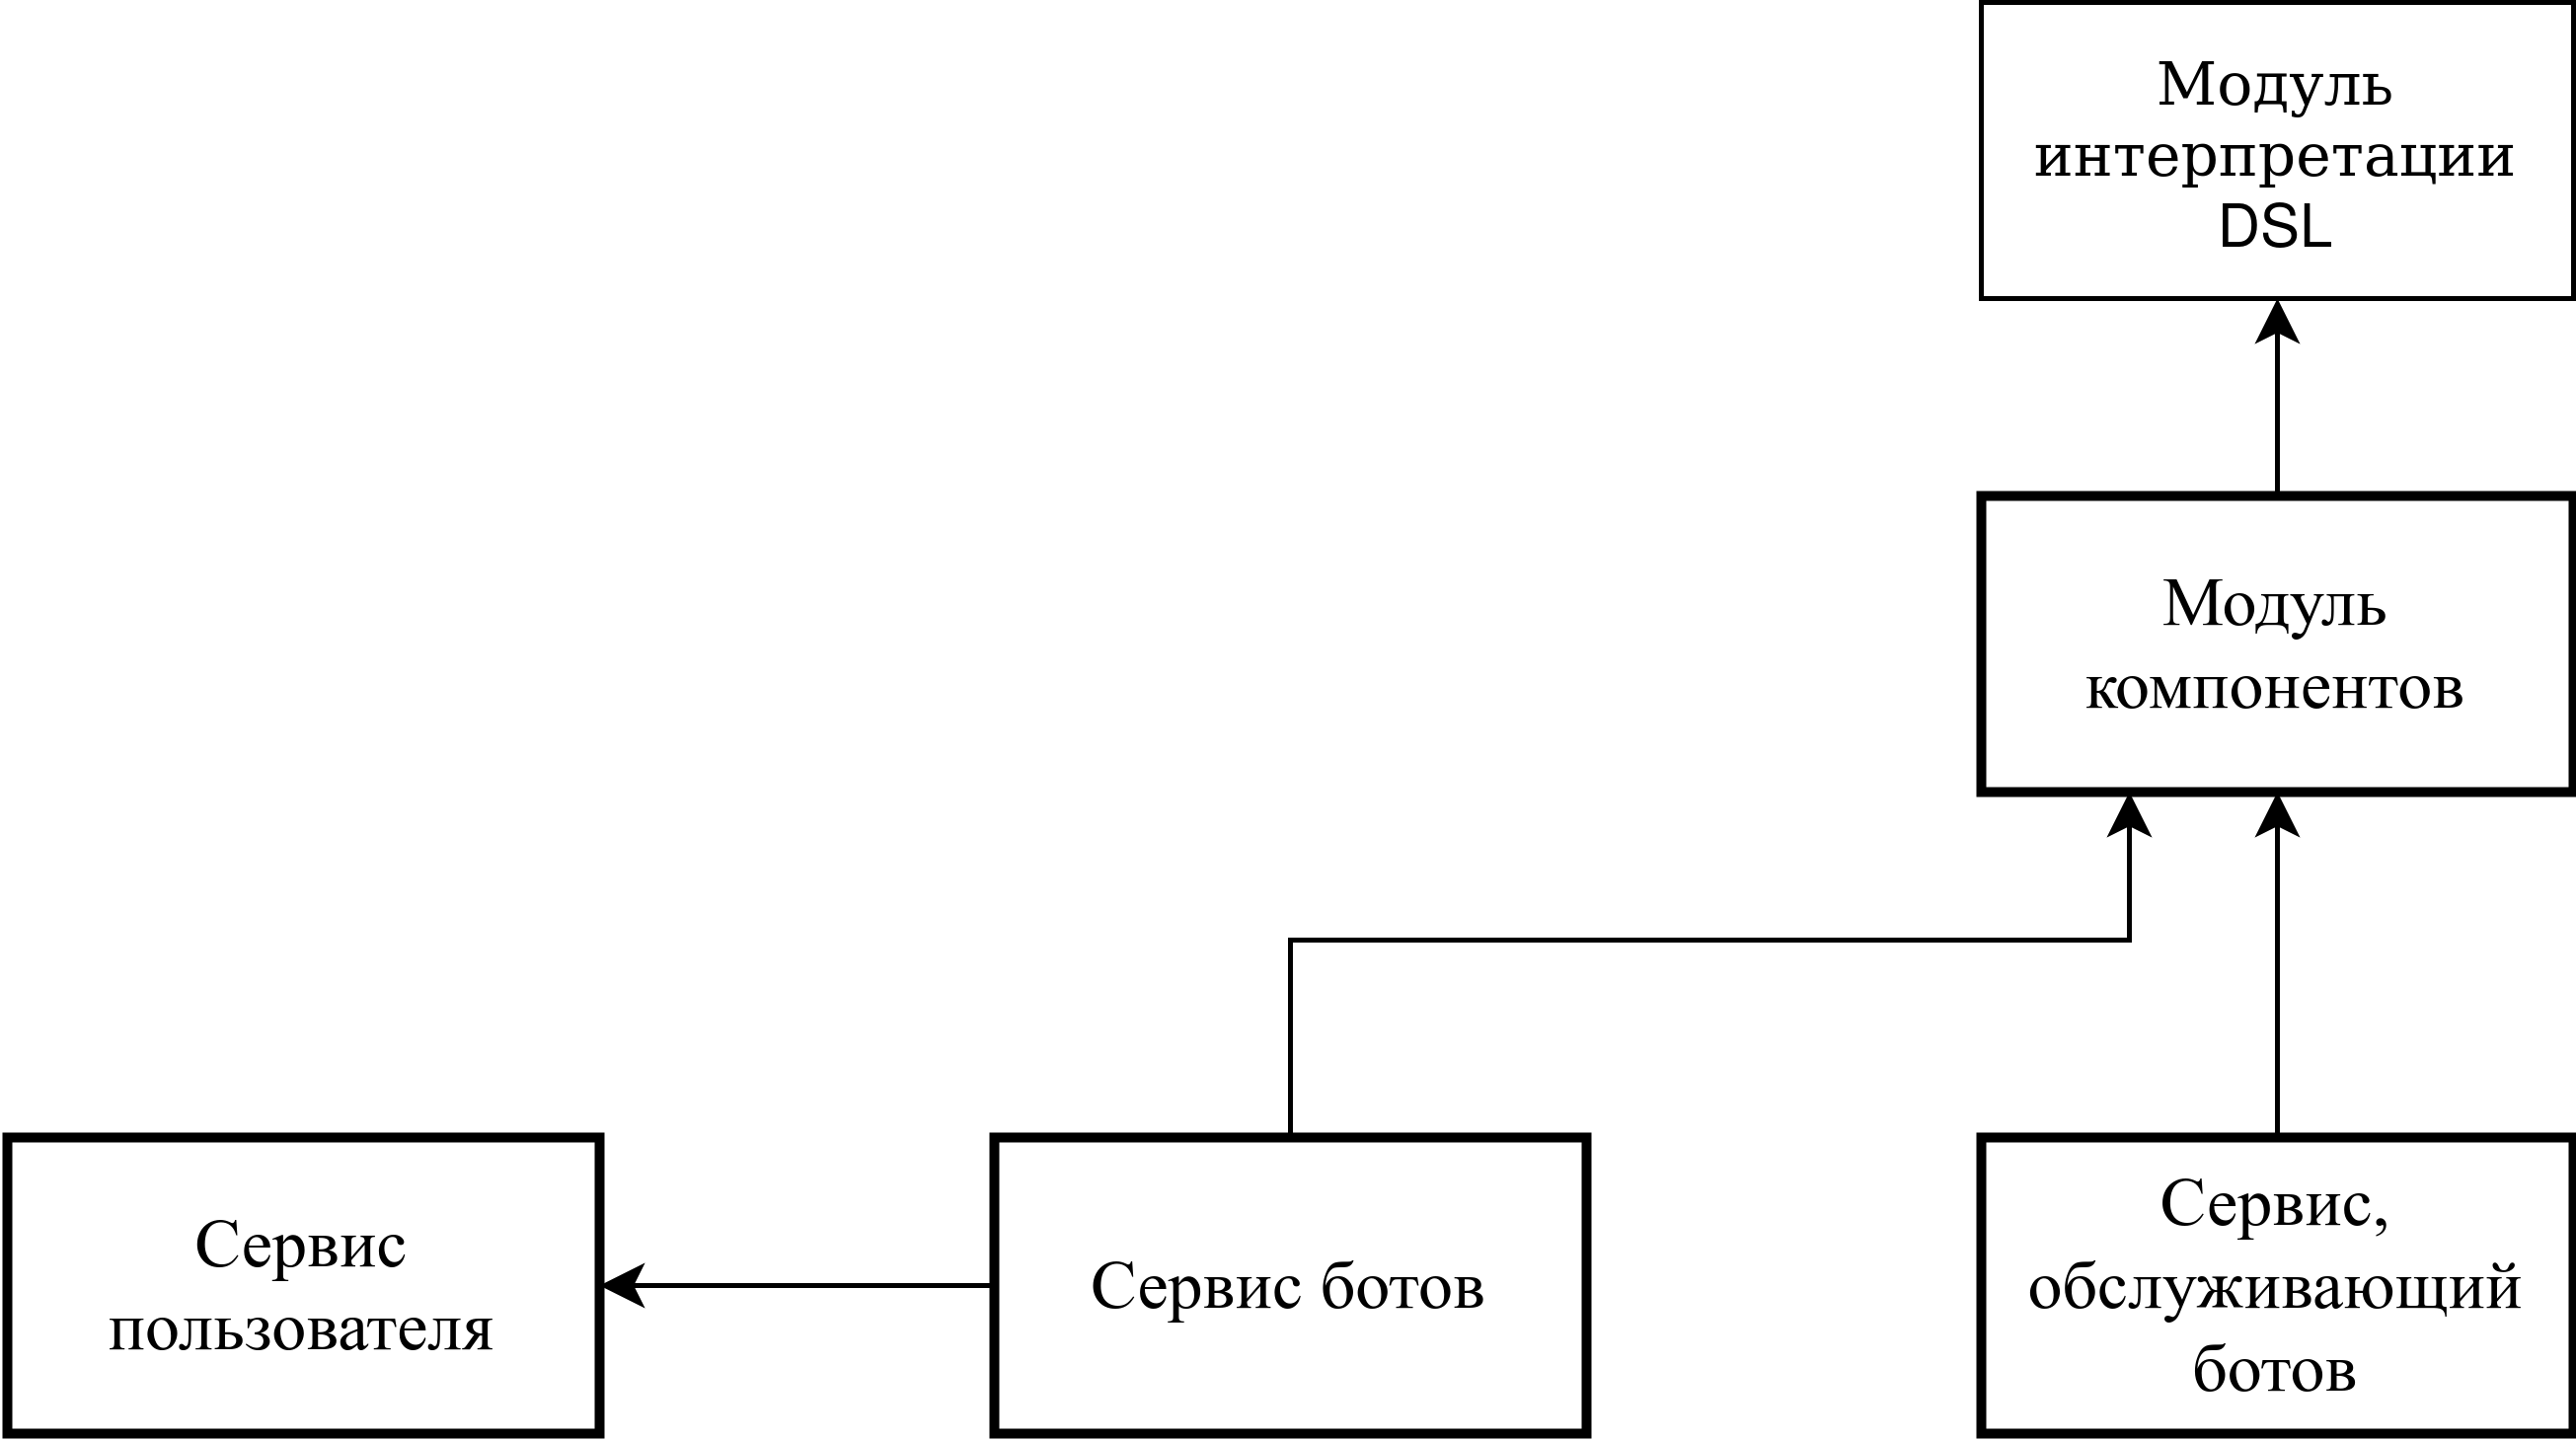
\includegraphics[width=0.8\textwidth]{structures/server/mod}
	\caption{Модульная структура серверной части конструктора}
	\label{f:mod-server-struct}
\end{figure}

Сервис ботов зависит от сервиса пользователей, который предоставляет
первому методы для авторизации пользователя. Также сервис ботов зависит
от модуля компонентов, который описывает структуры компонентов и
реализует их логику выполнения.

Для выполнения логики ботов сервис, обслуживающий ботов, вызывает
методы из модуля компонентов.

\subsubsection{Структура модуля компонентов}

Модуль компонентов состоит из следующих подмодулей:
\begin{itemize}
	\item подмодуль компонентов;
	\item подмодуль контекста;
	\item подмодуль исполнителя;
	\item подмодуль ввода-вывода.
\end{itemize}

Структура модуля компонентов представлена на рисунке~\ref{f:mod-comp-struct}.

\begin{figure}[ht]
	\centering
	\vspace{\toppaddingoffigure}
	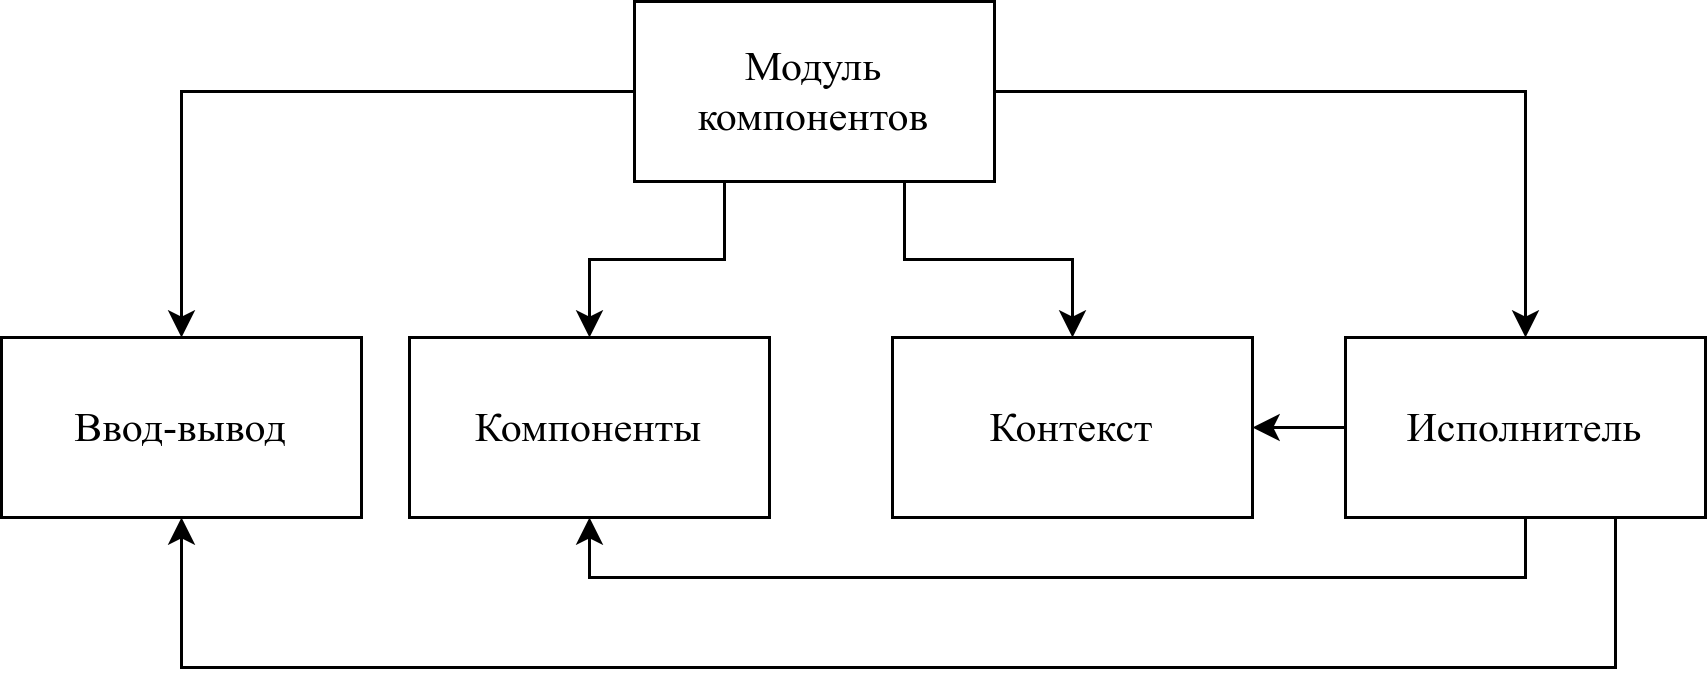
\includegraphics[width=0.8\textwidth]{structures/server/mod-comp}
	\caption{Структура модуля компонентов}
	\label{f:mod-comp-struct}
\end{figure}

Подмодуль компонентов содержит структуру и реализацию логики
компонентов. Каждый компонент реализует общий интерфейс компонента,
который определен в данном подмодуле.

В данном подмодуле определены следующие компоненты:
\begin{itemize}
	\item 	компонент ввода текста;
	\item 	компонент отправки сообщения;
	\item 	компонент вывода кнопок;
	\item 	компонент форматирования;
	\item 	компонент точки входа;
	\item 	компонент условия.
\end{itemize}

Подмодуль ввода-вывода предоставляет интерфейс, через который
окружение обменивается данными с рядом компонентов.

Подмодуль контекста содержит методы для работы с контекстом.
Контекст в рамках бота – память, с которой работают компоненты:
компоненты получают из контекста данные для выполнения и записывают в
него результат.

Исполнитель представляет собой объект, который содержит в себе
контекст и интерфейс ввода-вывода. Через него происходит выполнение
компонентов.


\subsubsection{Алгоритмы функционирования серверной части конструктора}

Пользователь конструктора взаимодействует с сервисом ботом, который
контролирует изменение данных и состояние ботов.
Схема алгоритма обработки запросов от пользователей сервиса ботов
представлен на рисунке~\ref{f:bot-service-alg}.

\begin{figure}[hp]
	\centering
	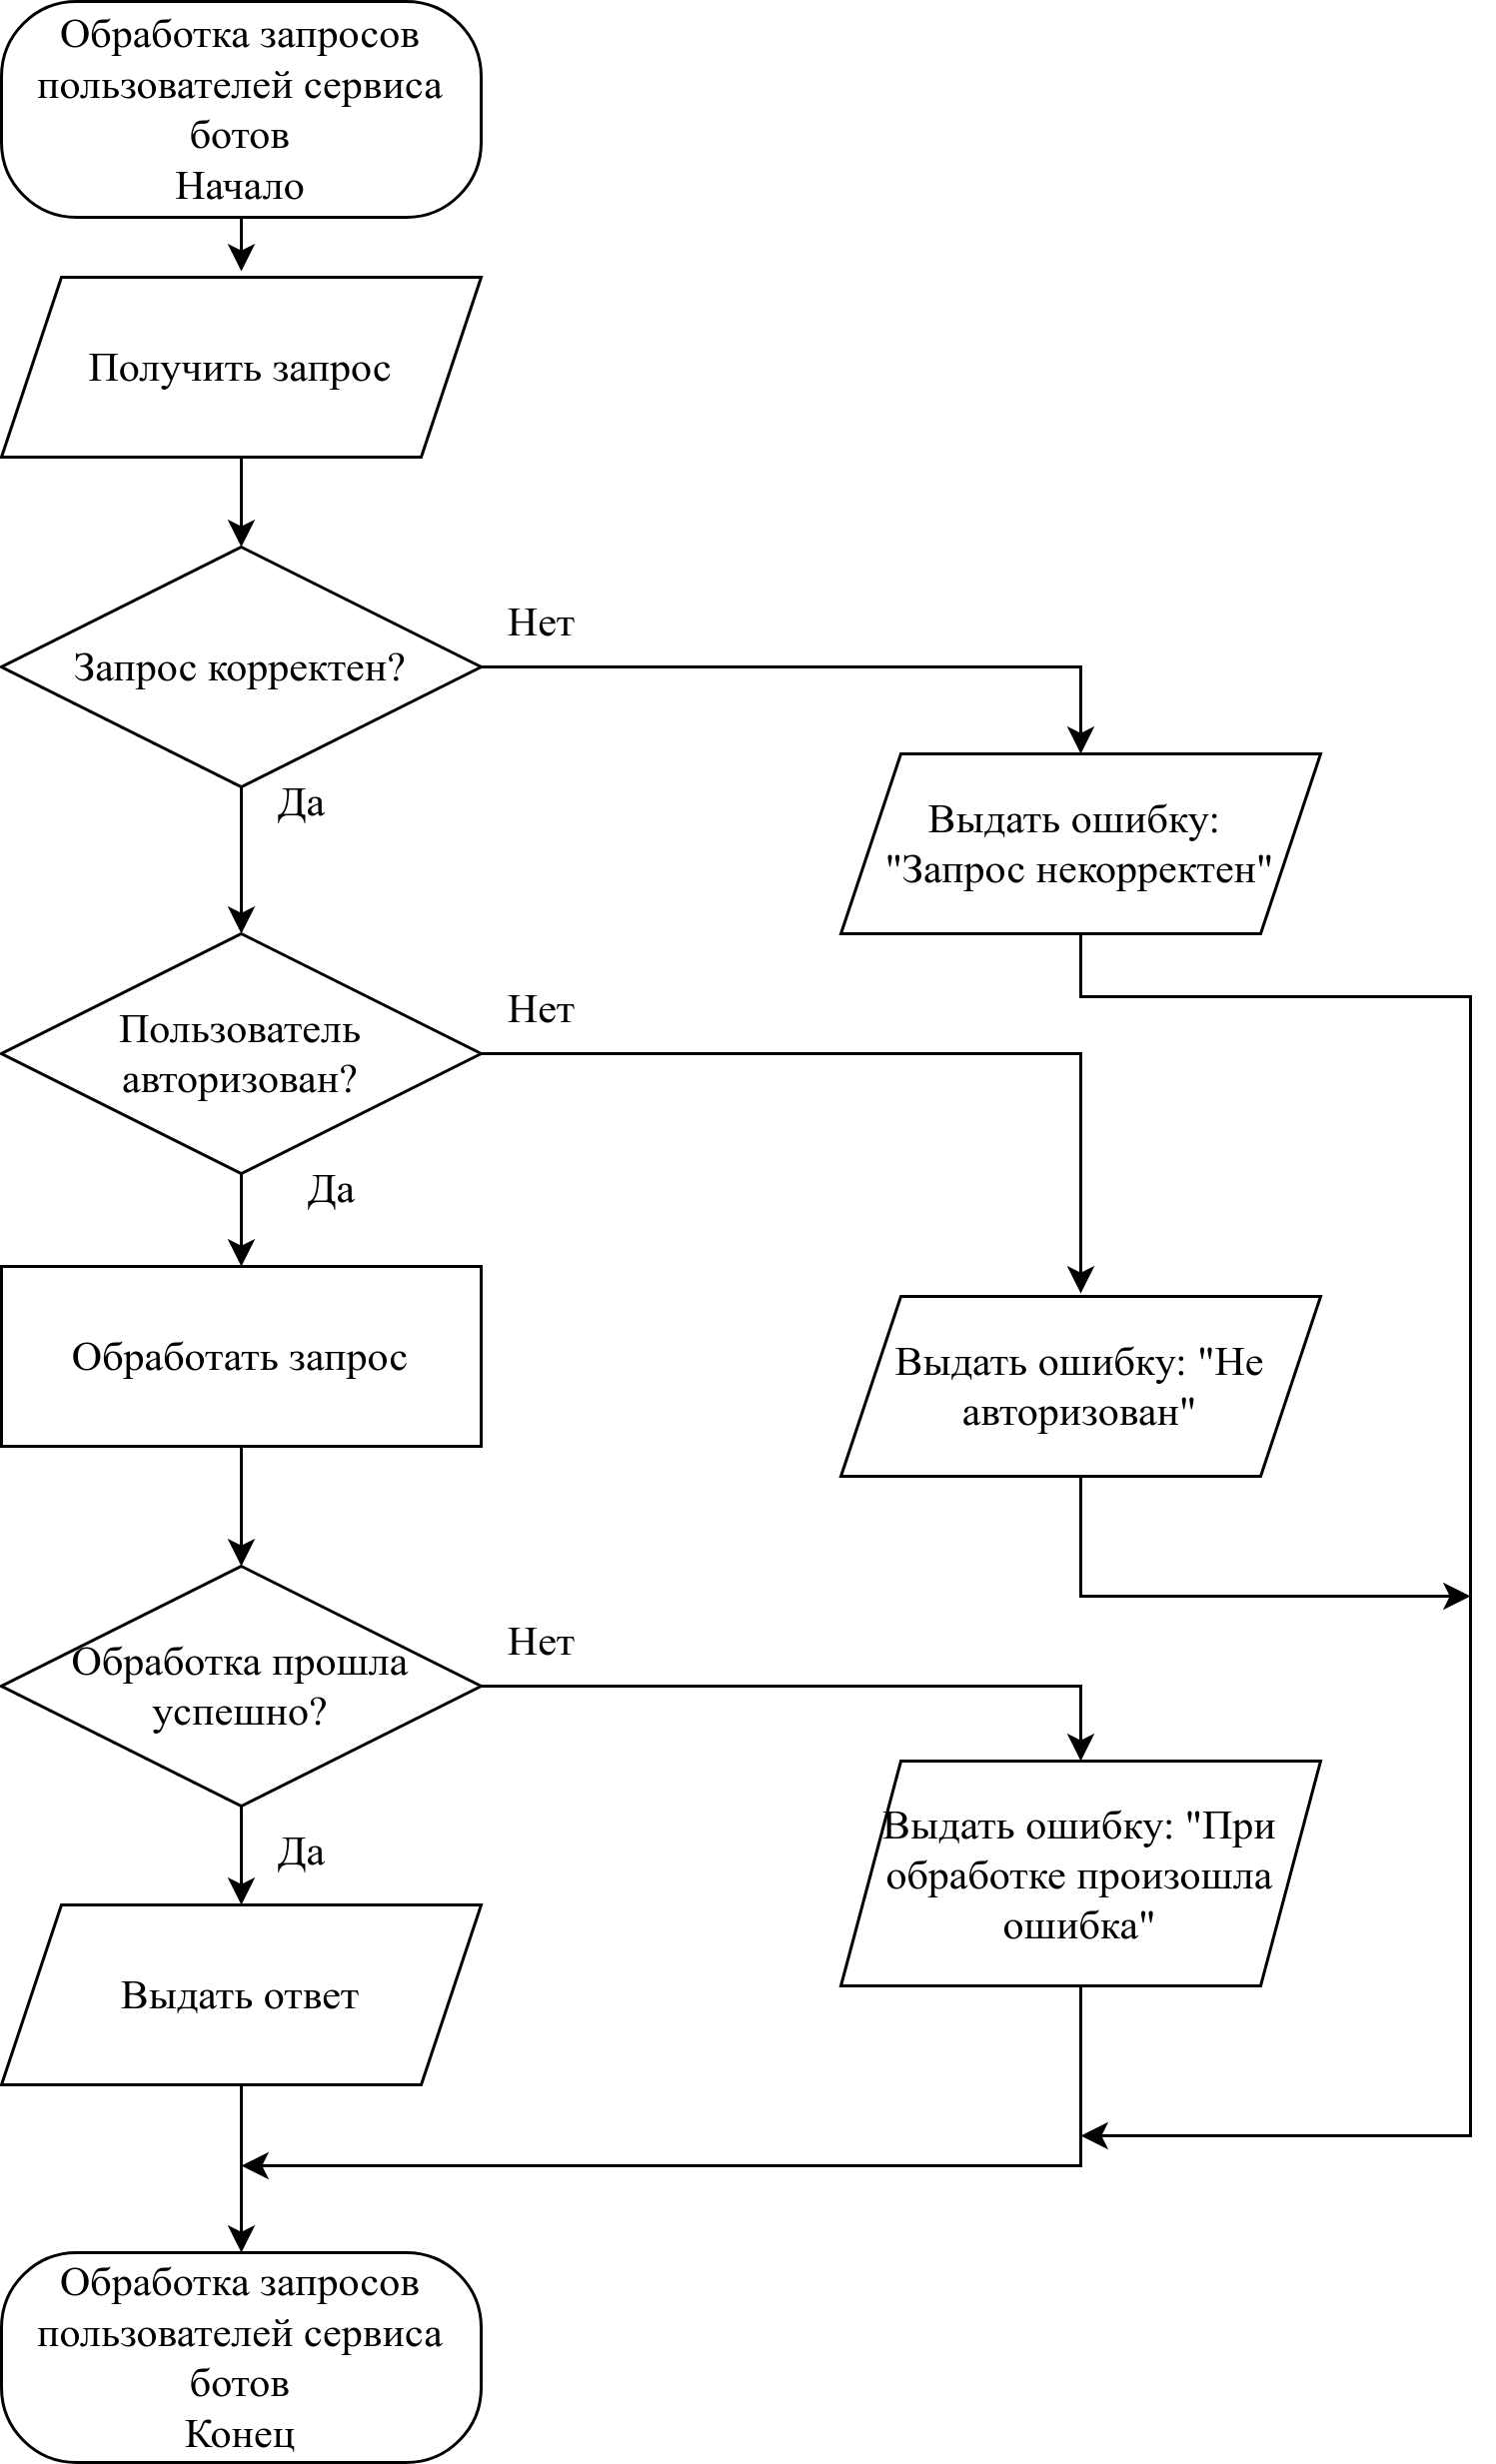
\includegraphics[height=0.9\textheight]{bot-service-alg}
	\caption{Схема алгоритма обработки запросов от пользователей сервиса ботов}
	\label{f:bot-service-alg}
\end{figure}

При получении запроса проверяется его корректность.
Если запрос не корректен, например, такое обращение не доступно, то
выводится соответствующая ошибка. Чтобы обработка прошла успешно, пользователь
должен быть авторизован в системе. В случае успешной обработки запроса выдается
ответ, иначе - ошибка.


При взаимодействии Telegram пользователя с ботом происходит
отправка запросов сервису, обслуживающему ботов, который в дальнейшем
обрабатывает данное событие. Схема алгоритма обработки запросов от
пользователя бота представлен на рисунке~\ref{f:bot-worker-alg}.


\begin{figure}[hp]
	\centering
	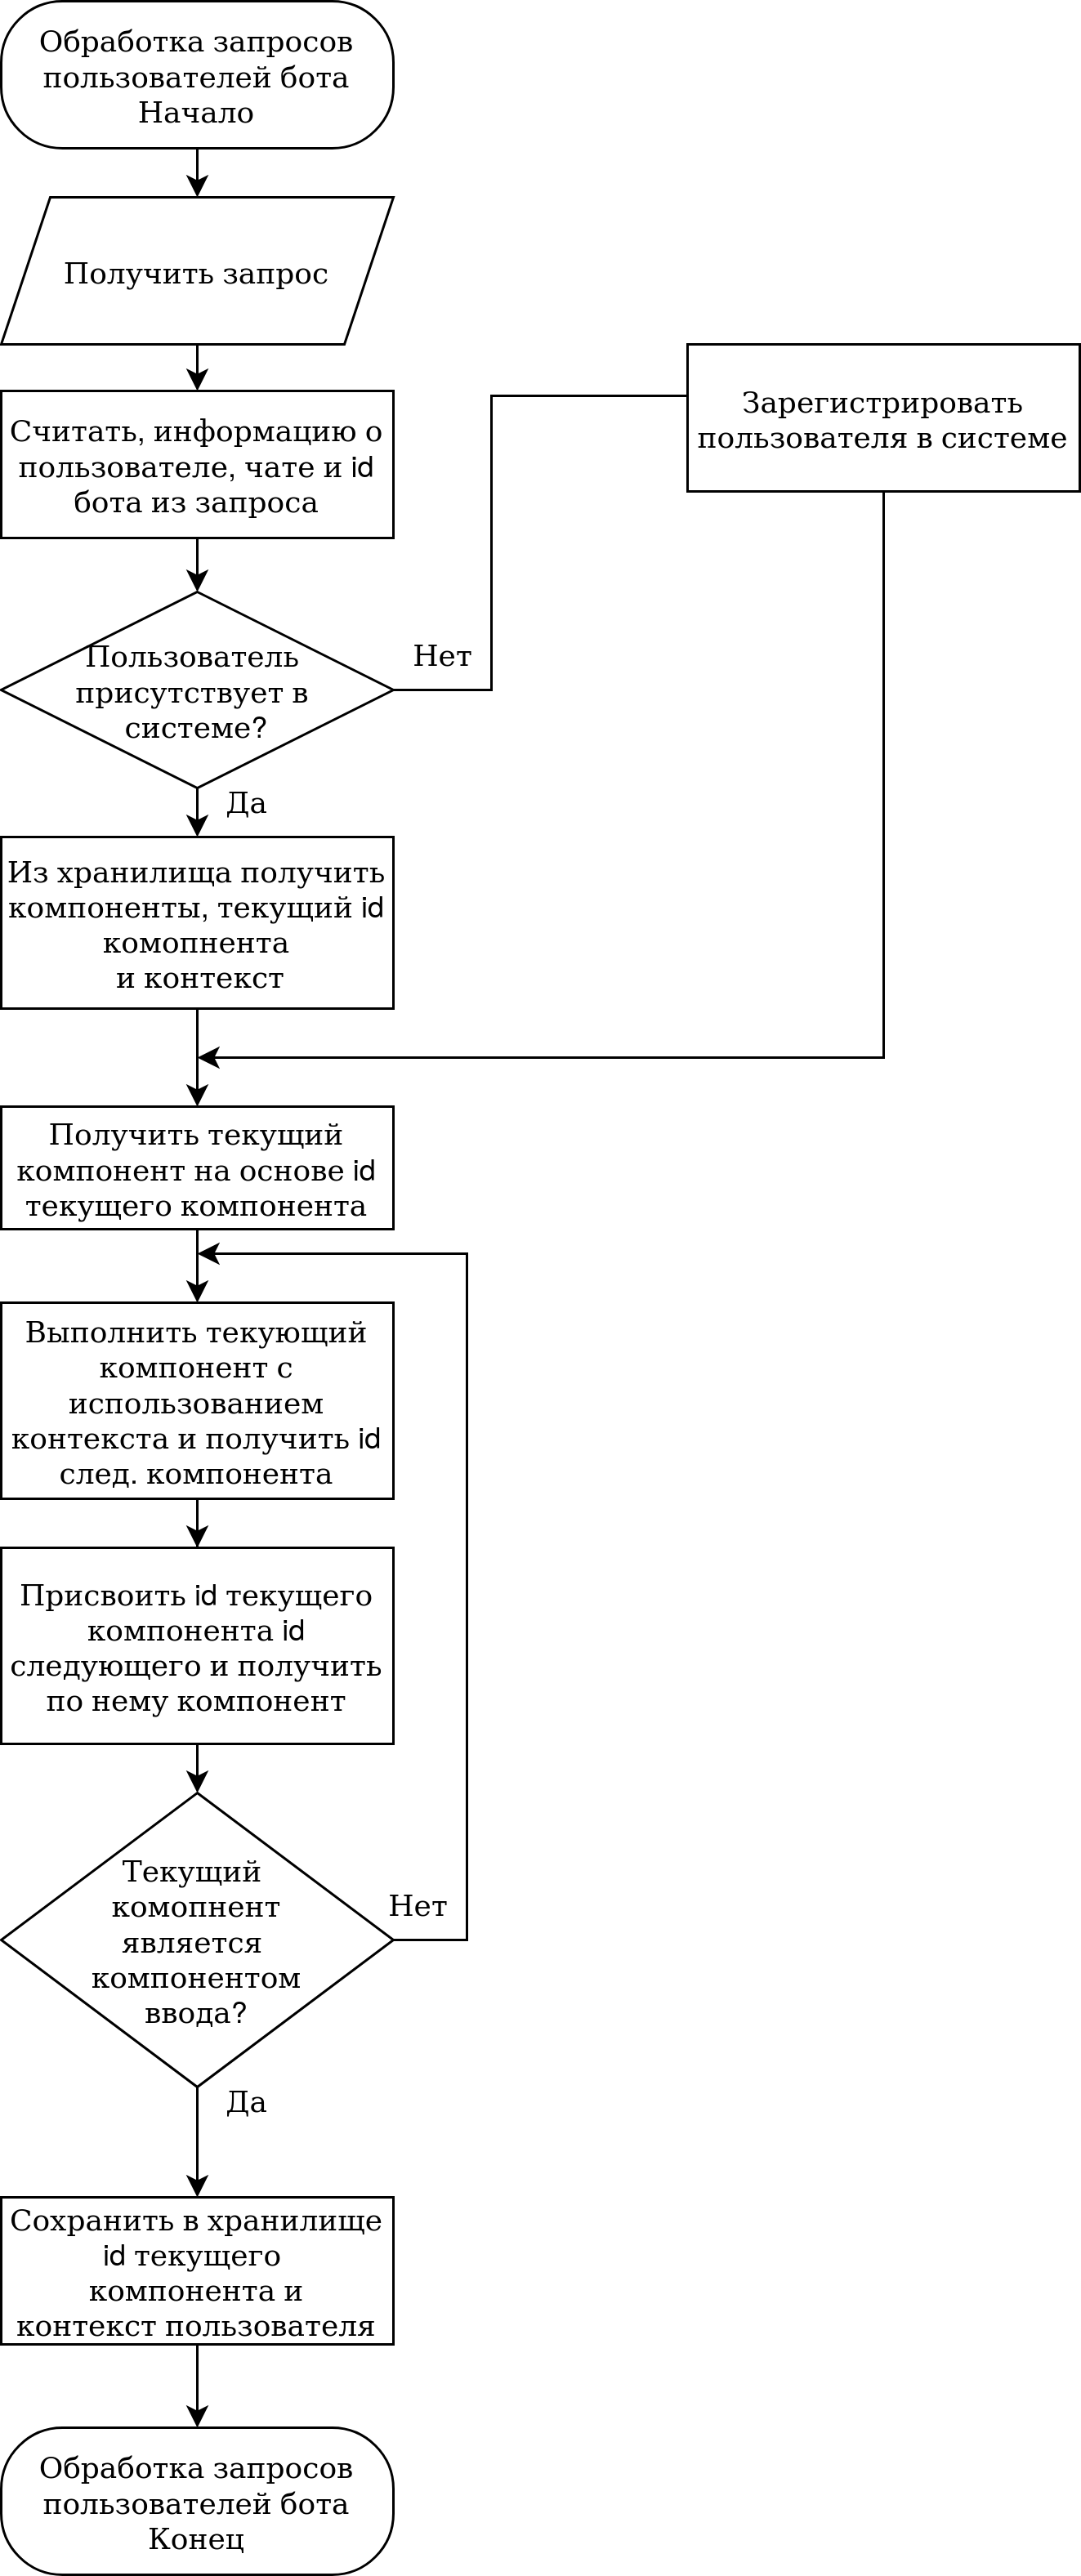
\includegraphics[height=0.9\textheight]{bot-worker-alg}
	\caption{Схема алгоритма обработки запросов от пользователей ботов}
	\label{f:bot-worker-alg}
\end{figure}

При принятии события сервисом происходит считывание следующих
данных:
\begin{itemize}
	\item информация о пользователе;
	\item информация о чате;
	\item id бота, от которого пришло сообщение.
\end{itemize}

На основе этих данных из хранилища идёт получение следующих
данных:
\begin{itemize}
	\item контекст пользователя;
	\item id текущего компонента пользователя;
	\item компонентов бота.
\end{itemize}

На основании id текущего компонента происходит получение текущего
компонента, который затем выполняется. Результат выполнения представляет
собой id следующего компонента, который присваивается текущему.

На основании следующего компонента принимается решение: если
компонент ожидает ввода каких-либо данных, то алгоритм заканчивается с
сохранением контекста и id текущего компонента, иначе идет выполнение
следующего компонента.

\newpage

\input{pages/content/struct/protection}


\subsection{Программная реализация клиентской части конструктора}

В данном подразделе обосновывается выбор инструментов
разработки клиентской части конструктора, а также демонстрируется
итоговый дизайн пользовательского интерфейса.

\input{pages/content/implementation/client/tools}
\input{pages/content/implementation/client/interface}


\newpage

\subsection{Пример использования}


Для демонстрации работы приложения был создан небольшой бот, который
просит ввести пользователя его имя и после выводит приветствие с использованием
данного имени.
Экранные формы примера работы приложения представлены на рисунках~
\ref{f:example:editor}-\ref{f:example:telegram}.

\begin{figure}[ht]
	\centering
	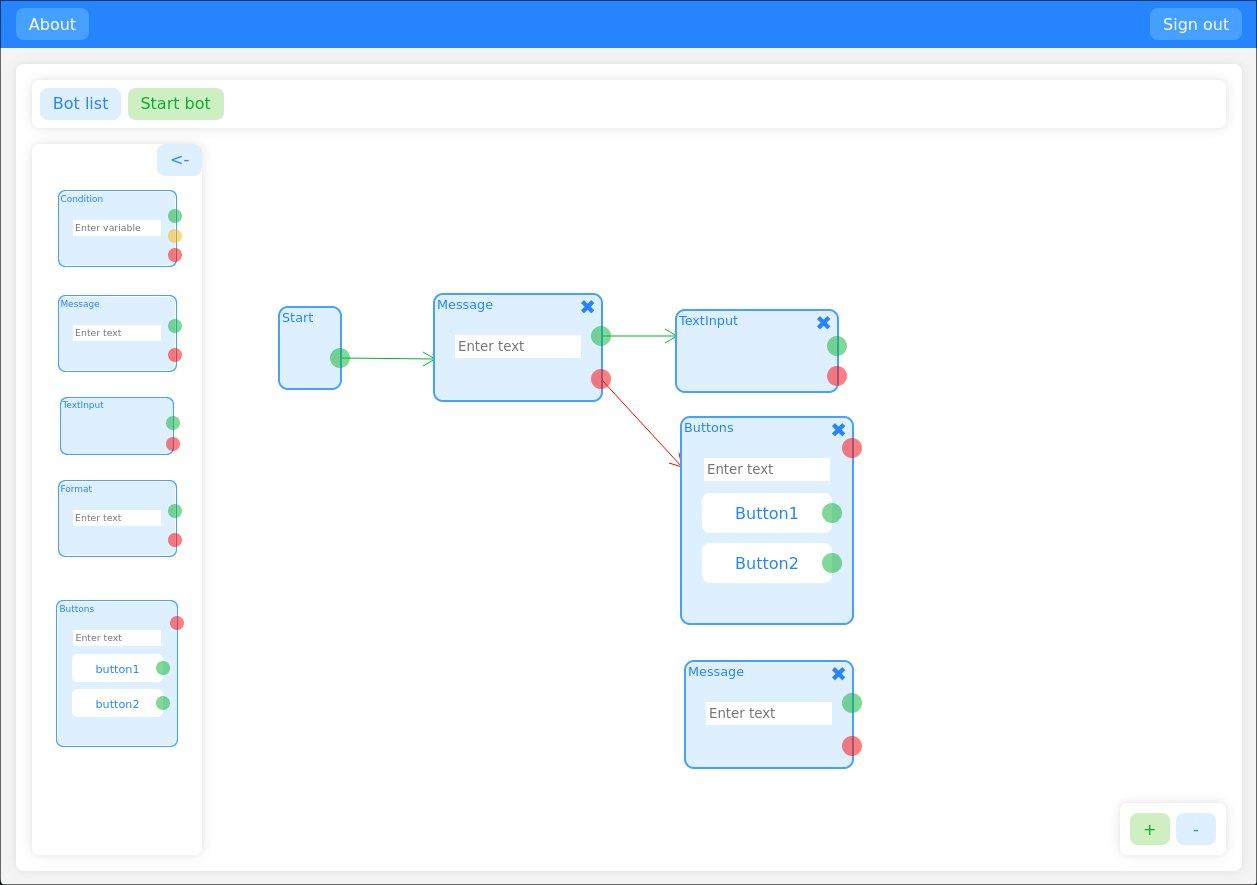
\includegraphics[width=\textwidth]{/example/editor}
	\caption{Построение структуры бота}
	\label{f:example:editor}
\end{figure}

\begin{figure}[ht]
	\centering
	
\includegraphics[width=0.9\textwidth]{/example/telegram}
	\caption{Использование созданного бота}
	\label{f:example:telegram}
\end{figure}




\newpage

\section*{Выводы}

В данном разделе были рассмотрены основные
инструменты и средства, используемые при создании
конструктора. Были рассмотрены аналоги, их плюсы и
минусы.

Был выбран формат передаваемых данных между серверной и клиентской
частями конструктора. У серверной части были выделены и разработаны
программные интерфейсы,
благодаря которым клиентская часть может обмениваться данными с сервисами.

На основе разработанных структур приложения, алгоритмов
функционирования и диаграмм состояний была выполнена программная реализация конструктора.
Листинг кода представлен в приложении \ref{ax:listing}.


\newpage

\csection{Заключение}

В ходе выполнения курсового проекта была выявлена структура
серверной части для конструктора Telegram ботов, предоставляющая собой
набор сервисов. Сервисы предоставляют программный интерфейс для
управления конструктором.

Для авторизации и реализации компонентов были выделены отдельные
модули. Модуль компонентов был также разбит на подмодули, которые
предоставляют интерфейсы для исполнения компонентов.

Был определен алгоритм обработки запросов пользователей бота,
который заключается в выполнении компонентов и сохранения текущего
состояния контекста пользователя бота после обработки.

Для разработки были выбраны оптимальные инструменты и определен
формат передаваемых данных, также разработан интерфейс для работы с
сервисами, который работает по протоколу HTTP.

По разработанной структуре была реализована серверная часть
конструктора Telegram ботов.


В ходе выполнения курсового проекта была выявлена структура
клиентской части для конструктора Telegram ботов, предоставляющая собой
набор страниц, с помощью которых пользователь может взаимодействовать с
конструктором.

Представлена модульная и компонентная структуры визуального
редактора. Модульная структура позволила выделить определенные
функциональные блоки редактора – набор структур и функций, которые
ответственны за определенную часть редактора; компонентная структура
помогла представить редактор как набор связанных компонентов в виде
дерева.

Была разработана диаграмма состояний для клиентской части
конструктора и редактора ботов, показывающая их поведение при действиях
пользователя.

Для разработки были выбраны оптимальные инструменты, определены
формат и структуры передаваемых данных.

По разработанной структуре была реализована клиентская часть
конструктора Telegram ботов.

\docappendix{Листинг кода}

\begin{lstlisting}
var a = 1;
var b = 10;
var c = 123;
var d = a + b + c;

some_function(a, b, c);
\end{lstlisting}


\docappendix[справочное]{Какое-то справочное приложение}


Содержимое приложения


}{
	% Привер файла содержимого документа
% Измените подключаемые файлы в зависимости от вашей структуры документа

\csection{Введение}

В современном мире стали популярными такие приложения для
быстрого общения как мессенджеры. Таких приложений достаточно много, но
большинство пользователей сети интернет все чаще отдают предпочтение
мессенджеру Telegram как наиболее удобному и надежному.

У Telegram имеется удобное API для создания ботов. Бот способен
выполнять определенные команды, заданные пользователем через интерфейс
Telegram. Данный функционал вполне может удовлетворять потребности
компании в предоставлении некоторых услуг в разных сферах. Например,
спортивные залы являются одной из таких сфер.

Создание ботов — это трудоемкий процесс, требующий
квалифицированных программистов, что довольно затратно для бизнеса.

Для решения данной проблемы существуют конструкторы Telegram-ботов, которые
предоставляют функции создания, редактирования и управления ботами.
К сожалению, большинство таких конструкторов предоставляют ограниченный функционал
при бесплатном использовании, а также имеют закрытые
способы хранения данных клиентов. Поэтому было принято решение выполнить анализ и
разработать конструктор Telegram-ботов без данных недостатков.


\pagebreak




\section{Анализ предметной области}

\subsection{Машина времени}

Машина времени является гипотетическим устройством, способным перемещаться во времени, обеспечивая возможность путешествия в прошлое или будущее. В связи с этим, анализ предметной области машины времени включает следующие аспекты:


\begin{enumerate}
	\item физические принципы: необходимо изучить теоретические основы, согласно которым могла бы функционировать машина времени. Это может включать обсуждение специальной теории относительности, черных дыр, петель времени и других концепций из физики;

	\item технические особенности: рассмотрим возможные способы построения и дизайна машины времени. Какие технологии или материалы могут быть использованы для ее создания? Какие опасности или препятствия могут возникнуть при ее конструировании?

	\item парадоксы времени: проанализируем различные парадоксы, которые могут возникнуть при использовании машины времени, такие как "парадокс дедушки" или "парадокс самовыполнения". Какие последствия они могут иметь для временных путешественников?

	\item этические и социальные аспекты: обсудим влияние машины времени на общество и индивидуума. Какие этические вопросы возникают при использовании данной технологии? Какие последствия она может иметь для личной и мировой истории?

	\item возможные приложения: рассмотрим потенциальные области применения машины времени, такие как исследования истории, изменение прошлого или будущего, предсказание событий и т. д.
\end{enumerate}

\subsection{Сравнение аналогов}

Машина времени 1:
\begin{itemize}
	\item перемещает человека в прошлое или будущее;
	\item имеет ограничение по количеству путешествий во времени;
	\item не поддерживает контроль точного места приземления.
\end{itemize}

Машина времени 2:
\begin{itemize}
	\item позволяет путешествовать во времени как в прошлое, так и в будущее;
	\item имеет более сложную систему навигации и управления;
	\item предоставляет дополнительные возможности и функции.
\end{itemize}

Машина времени 3:
\begin{itemize}
	\item позволяет точно указывать дату, время и место для путешествия;
	\item обладает самой передовой технологией и функционалом;
	\item эффективнее и безопаснее других машин времени.
\end{itemize}

Эти машины времени можно сравнивать через их уникальные особенности, функционал, надежность и возможности путешествия. Каждая из них обладает своими преимуществами и ограничениями, что делает их различными в использовани

В таблице \ref{t:comp-an} представлено сравнение аналагов.

\begin{table}[ht]
	\Large
	\caption{Сравнение аналогов}
	\label{t:comp-an}
	\centering
	\begin{tabularx}{\textwidth}{|X|c|c|c|}
		\hline
		Критерии \textbackslash\ Аналоги & Машина времени 1 & Машина времени 2 & Машина времени 3 \\
		\hline
		Критерий 1
		                                 & нет              & да               & да               \\
		\hline
		Критерий 2
		                                 & нет              & да               & да               \\
		\hline
		Критерий 3
		                                 & да               & да               & нет              \\
		\hline
		Критерий 4
		                                 & нет              & нет              & да               \\
		\hline
	\end{tabularx}
	\vspace{\bottompaddingoftable}
\end{table}

Таким образом разработка машины времени является актуальной.

\section*{Выводы}


Анализ предметной области машины времени требует не только фантазии и творческого мышления, но и глубоких знаний в области физики, философии, этики и технологии.





\subsection{Расширенное техническое задание}

В данном разделе представлено техническое задание на разработку
конструктора Telegram-ботов.

\subsubsection{Краткая характеристика области применения}

Программа предназначена для создания
Telegram-ботов, которые будут удовлетворять
потребности клиентов в создании их бизнес-решений.


\subsubsection{Основание для разработки}

Функциональным назначением программы является предоставление
клиентам возможности создания Telegram-ботов при помощи визуального редактора и
без глубоких знаний языков программирования.

Программа должна эксплуатироваться на серверах клиента.
Для использования конечному пользователю предъявляются требования знания процесса
развёртывания серверных приложений.


\subsubsection{Требования к структуре}

Конструктор должен состоять из двух частей: серверной и клиентской.
Серверная часть должна обеспечивать основной функционал конструктора.
Клиентская часть предоставляет собой удобный пользовательский интерфейс.

\subsubsection{Требования к серверной части конструктора}

В подпунктах данного раздела описываются требования к серверной части конструктора.

\paragraph{Требования к функциональным характеристикам}

Серверная часть конструктора должна предоставлять программный
интерфейс, который обеспечивает выполнение следующих функций:
\begin{itemize}
	\item регистрация пользователей;
	\item аутентификация пользователей;
	\item создание ботов;
	\item вывод списка ботов;
	\item запуск и остановку ботов;
	\item добавлять компоненты;
	\item удалять компоненты;
	\item редактировать содержимое компонента;
	\item соединять компоненты;
	\item обслуживать запросы пользователей от запущенных ботов.
\end{itemize}

\paragraph{Требования к предоставляемому программному интерфейсу}

Программный интерфейс, который предоставляется серверной частью
конструктора должен удовлетворять следующим требованиям:
\begin{itemize}
	\item должен быть прост и интуитивен;
	\item должен быть надежен и доступен;
	\item должен включать возможность аутентификации и авторизации;
	\item должен обрабатывать возможные ошибки при запросе
	      пользователя.
\end{itemize}

\paragraph{Требования к параметрам технических и программных средств}

В состав технических средств должен входить компьютер, включающий
в тебя:
\begin{itemize}
	\item 64-разрядный процессор с тактовой частотой не менее 1.0 ГГц;
	\item не менее 4 гигабайт оперативной памяти;
	\item не менее 1 гигабайт свободного дискового пространства;
	\item сетевую карту.
\end{itemize}

Также для работы севера требуется предустановленная операционная
система на базе ядра Linux: Ubuntu 18.04 или старше, Debian 10 или старше.

\subsubsection{Требования к клиентской части конструктора}

В подпунктах данного раздела описываются требования к клиентской части конструктора.


\paragraph{Требования к функциональным характеристикам}

Клиентская часть конструктора должна иметь возможность
формировать и отправлять данные и запросы для выполнения следующих
функций:
\begin{itemize}
	\item регистрация пользователей;
	\item аутентификация пользователей;
	\item создание ботов;
	\item вывод списка ботов;
	\item запуск и остановку ботов;
	\item редактирование ботов.
\end{itemize}

Для работы с содержимым ботов клиентская часть должна содержать
визуальный редактор. Редактор предоставляет пользовательский интерфейс
для выполнения следующих функций:
\begin{itemize}
	\item добавление компонентов;
	\item удаление компонентов;
	\item редактирование содержимого компонентов;
	\item соединение компонентов.
\end{itemize}


\paragraph{Требования к пользовательскому интерфейсу}

Интерфейс конструктора Telegram ботов должен состоять из страниц,
содержащих разные визуальные элементы, которые предоставляют
пользователям возможность взаимодействовать с конструктором.

Также интерфейс должен обеспечивать
наглядное, интуитивно понятное представление.

\paragraph{Требования к клиентскому программному обеспечению}

Клиентская часть конструктора Telegram-ботов должна быть доступна для
полнофункционального использования с помощью следующих браузеров:
\begin{itemize}
	\item Edge 88.0 и выше;
	\item Opera 43.0 и выше;
	\item Mozilla Firefox 55.0;
	\item Google Chrome 64.0 и выше.
\end{itemize}

\subsubsection{Стадии разработки}

Разработка должна быть проведена в следующих стадиях:
\begin{itemize}
	\item разработка технического задания;
	\item проектирование структуры серверной части конструктора;
	\item проектирование структуры клиентской части конструктора;
	\item программная реализация серверной части конструктора;
	\item программная реализация клиентской части конструктора.
\end{itemize}


\newpage

\section{Структура машины времени}

Структура машины времени представлена на рисунке~\ref{f:time-machine}.


\begin{figure}[ht]
	\centering
	\vspace{\toppaddingoffigure}
	
\includegraphics[width=0.7\textwidth]{time-machine}
	\caption{Структура машины времени}
	\label{f:time-machine}
\end{figure}


Разработка структуры машины времени является сложной задачей, поскольку такое устройство находится за пределами существующих научных и инженерных возможностей. Однако, если мы предположим, что машина времени возможна, то ее структура, вероятно, будет иметь следующие основные компоненты:

\begin{enumerate}
	\item часовой механизм: стандартный механизм, который управляет передвижением во времени, аналогично тому, как часовой механизм контролирует передвижение стрелок на циферблате часов;

	\item энергетический источник: мощный источник энергии, способный обеспечить работу машины времени и перемещение объектов во времени;

	\item контрольная система: комплекс алгоритмов и программного обеспечения, которые контролируют точное время и координируют перемещение во времени;

	\item защитные механизмы: системы, предотвращающие нежелательное перемещение во времени или обеспечивающие безопасность при использовании машины времени;

	\item интерфейс пользователя: устройства ввода и вывода, позволяющие пользователю программировать желаемые временные точки или координировать перемещение во времени;

	\item материалы и конструкция: специальные материалы и компоненты, обеспечивающие устойчивость и работоспособность машины времени.
\end{enumerate}

Хотя это очень упрощенное описание возможной структуры машины времени, это может помочь представить основные компоненты, которые потребуются для того, чтобы создать такое устройство. Однако необходимо помнить, что вышеописанная концепция является вымышленной и не имеет научного обоснования.


Пример ссылки на источник \refref{ref:num-methods}.

Пример еще ссылки на источник \refref{ref:time-series-analysis}.

\subsection{Расчёты}

Расчёты представлены ниже

\begin{gather}
	a = \tan(\frac{\alpha}{2})*a*\pi, \\
	\bigtriangleup b = \cos(\beta)*a, \\
	c = \sin{\beta}.
\end{gather}


\examplecommand

\docappendix{Листинг кода}

\begin{lstlisting}
var a = 1;
var b = 10;
var c = 123;
var d = a + b + c;

some_function(a, b, c);
\end{lstlisting}


\docappendix[справочное]{Какое-то справочное приложение}


Содержимое приложения


}


\end{document}
